% \newcommand{\prototitle}{Versuch 2 - Statistik}
% \newcommand{\Fachbereich}{Praktikum Messtechnik}
% \input{../packages/tu_header}

\newcommand{\institut}{Institut f\"ur Telekommunikationssysteme}
\newcommand{\fachgebiet}{Nachrichten\"ubertragung}
\newcommand{\veranstaltung}{Praktikum Nachrichten\"ubertragung}
\newcommand{\pdfautor}{\"Ozg\"u Dogan (326 048), Boris Henckell (325 779)}
\newcommand{\autor}{\"Ozg\"u Dogan (326 048)\\ Boris Henckell (325 779)}
\newcommand{\gruppe}{Gruppe: D03}
%\newcommand{\betreuer}{Betreuer: Mahmoud Felk}


\newcommand{\pdftitle}{Nachrichten\"ubertragung\ Praktikum\ 05}
\newcommand{\prototitle}{Praktikum 05 \\ Pulscodemodulation und Quantisierung}


\input{../../packages/tu_header_8}
 \begin{document}

% \lstlistoflistings
\definecolor{darkgray}{rgb}{0.95,0.95,0.95}
\definecolor{darkolivegreen}{HTML}{01a801}
\definecolor{functionsBlue}{HTML}{32b9b9}
\definecolor{variableRed}{rgb}{1,0,0}
\definecolor{stringBrown}{HTML}{bc8e8e} % f geht nicht

\lstset{
        %\lstset{extendedchars=true} % Umlaute an der richtigen stelle und nicht am Anfang ausgeben
        %basicstyle=\footnotesize\ttfamily,
        basicstyle=\small,
        %
        inputencoding=utf8,
        %
        tabsize=4,
        showspaces=false,
        showtabs=false,
        showstringspaces=true, % no special string spaces
        %
        backgroundcolor=\color{darkgray}, % background
        stringstyle=\color{stringBrown}\fseries, % Strings
        keywordstyle=\color{functionsBlue}\bfseries, % keywords Blau
        identifierstyle=\color{variableRed}, % variablen
        commentstyle=\color{darkolivegreen}, %  comments
        %
        breaklines=true,
        %
        numbers=left,
        numberstyle=\tiny,
        stepnumber=1,
        numbersep=7pt,
        %
        frame=single,
        columns=flexible,
        %
        xleftmargin=-2cm,
        xrightmargin=-1.5cm,
        %
        language=Matlab
}

%---------------------------------------------------------------------
%---------------------------------------------------------------------
%---------------------------------------------------------------------


\section{Einleitung}
\begin{quote}
	
	In diesem Termin wird eine Pulscodemodulation (PCM) Übertragungstrecke
	aufgebaut und untersucht. Außerdem wird das Ausmaß von Quantisierungsfehlern
	bei der digitalen Übertragung, sowie das Leistungsdichtespektrum (LDS) dieser
	Fehler gemessen.

\end{quote}%beende Einleitung
%--------------------------------------------------------------------
%--------------------------------------------------------------------    

\section{Motivation}
\begin{quote}
	
	Ursprünglich wurden Signale wie Mess-, Audio- und Bildsignale ausschließlich in
	analoger Form übertragen. Durch diese Art der Übertragung treten aber
	Rauschstörungen, lineare Verzerrungen (Änderungen des Frequenzganges) und
	nichtlineare Verzerrungen (Klirr) auf, welche auf der Empfängerseite kaum
	verringert werden können. Diese Störungen treten bei der digitalen Übertragung
	kaum auf, oder können beliebig klein gehalten werden, weshalb analoge Signale
	verstärkt anhand digitaler Kanäle übetragen werden.\\
	Eine Art der digitalen Übertragung ist die Pulscodemodulation.
	
\end{quote} %section

%--------------------------------------------------------------------
%--------------------------------------------------------------------    


\section{Theorie}
\begin{quote}

	Eine Pulscodemodulation basiert auf das Abtasten und Codeworterzeugung eines
	analogen Signals. Dabei wird das analoge Signal mithilfe eines A/D-Wandlers
	digitalisiert, codiert und nach der Übertragung beim Empfänger decodiert und
	mit einem D/A-Wandler wieder in ein analoges Signal umgewandelt. Eine
	Kanalcodierung des Übertragungskanal kann dabei für zusätzlichen Fehlerschutz
	vor Übertragungsfehlern sorgen.\\
	
	\begin{figure}[H]
    \centering
        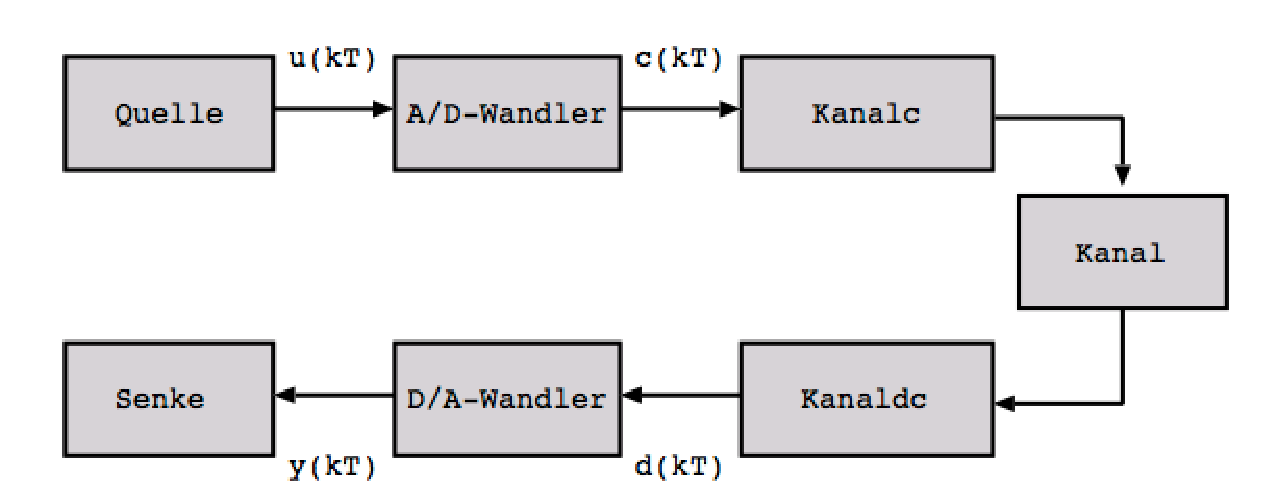
\includegraphics[scale=0.7, trim = 0cm 0cm 0cm 0cm, clip]{./Bilder/PCM-Uebertragung}
            \caption{PCM-Uebertragung}
            \cite{PCM-Uebertragung}
    \end{figure}
    
	
	Eine digitale Übertragung bietet viele Vorteile, wie zum Beispiel
	\begin{itemize}
		\item die Übertragungsqualität nimmt über weite Entfernungen durch den Einsatz
		von Regenerativverstärkern nicht ab
		\item die Multiplexbildung (z.B. TDM) ist vereinfacht
		\item es ist eine Integration von digitaler Übertragung und digitaler
		Vermittlung vorhanden
		\item die Wirtschaftlichkeit ist größer
		\item das Zusammenwirken mit digitalen Verfahren der Nachrichtenverarbeitung
		ist vereinfacht
		\item die Integration von Diensten ist möglich 
		\item es ist eine praktisch störungsfreie Übertragung durch Fehlerkorrekturen
		erreichbar
		\item und es besteht die Möglichkeit der Verschlüsselung um die Wahrung des
		Fernmeldegeheimnisses zu verbessern.
	\end{itemize}
	
	\vspace{1em}
	
	Die beiden Nachteile der digitalen Übertragung sind dagegen
	\begin{itemize}
		\item die Entstehung von Quantisierungfehlern
		\item und der erhöhte Bandbreitebedarf.
	\end{itemize}
	
	\vspace{0.5em}
	
	An dieser Stelle ist zu erwähnen, dass die Quantisierungfehler bei einer
	PCM-Übertragung relativ klein gehalten werden können und dass der höhere
	Bandbreitebedarf bei modernen digitalen Verfahren mit effizienten
	Quellencodierungen und mehrstufigen Übertragungen der Binärinformation nicht
	mehr auftritt.\\
	
	Bei der PCM-Übertragung wird das analoge Signal mit einer
	oberen Grenzfrequenz von $B_{Quelle}$ mit einer Abtastfrequenz von $f_T \geq 2
	\cdot B_{Quelle}$ abgetastet, wodurch ein PAM Signal mit den Abtastwerten im
	Abstand $T = \frac{1}{f_T}$ entsteht.\\
	Anhand eines Quantisierers wird diesen Werten jeweils eins von $M = 2^m$ möglichen wertdiskreten Signalen zugeordnet,
	deren Indizes in digitale Codewörter umgewandelt werden. Diese Codewörter sind
	typischerweise in binärer Form und bestehen aus $m = ld(M)$ Bit pro Abtastwert.
	Dabei einsteht eine Bitrate von
	
       \begin{equation*}
        	\begin{split}
        		R_{Bit} = f_T \cdot m \ \ \frac{bit}{s}
        	\end{split}
        \end{equation*}        
    
	\vspace{0.5em}
	   
	Zusammen ergeben der Abtaster, das Halteglied und der Quantisierer den
	A/D-Wandler bei der Digitalisierung eines analogen Signals.\\
	
	\begin{figure}[H]
    \centering
        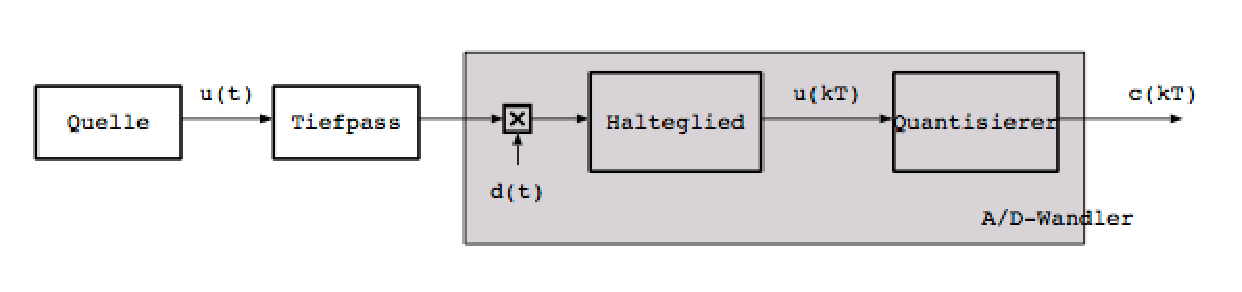
\includegraphics[scale=0.7, trim = 0cm 0cm 0cm 0cm, clip]{./Bilder/Digitalisierung_des_Signals}
            \caption{Blockschaltbild Digitalisierung eines Signals}
            \cite{Digitalisierung_des_Signals}
    \end{figure}
    
	Übertragen werden diese wertdiskreten Signale durch den digitalen Kanal, der
	sie bei fehlerfreier Übertragung eins zu eins an den Empfänger weitergibt. \\
	
	Dabei setzt sich der Kanal aus den Übertragungsschritten Umwandlung in
	binäre Signalelemente, Impulsformung und Modulation bishin zum Entscheider 
	auf der Empfangsseite zusammen.\\
	Für die Kanalbandbreite bei einer binären Übertragung eines PCM-modulierten
	Signals und einer Bitrate von $R_{Bit} = f_T \cdot m \ \ \frac{bit}{s}$ gilt:
	 
       \begin{equation*}
        	\begin{split}
        		B_{Kanal,binäre PCM} = \frac{R}{2} \cdot (1+r)  =  m \cdot
        		B_{Quelle} \cdot (1+r)
        	\end{split}
        \end{equation*}        
        
	\vspace{0.5em}
	    
	Das $r$ entspricht dem Flankenfaktor, welcher einen Wert von $0 < r \leq 1$
	annehmen kann. Man sieht, dass für eine fehlerfreie Übertragung mindestens die
	 $m$-fache Quellbandbreite benötigt wird. Dieser kann aber wiederum verringert werden, wenn die $M$-wertigen
	Quantisierungsausgangswerte nicht in $m$ binäre Codewörter umgewandelt werden,
	sondern in $N$-wertige Codewörter. Dadurch entsteht in der Rechnung ein
	zusätzlicher Faktor, welcher die Kanalbandbreite reduziert:
	
	 \begin{equation*}
        	\begin{split}
        		B_{Kanal,N-wertige PCM} = \frac{m}{ld(N)} \cdot B_{Quelle} \cdot (1+r)
        	\end{split}
      \end{equation*}     
	
	\vspace{0.5em}
	
	Die Decodierung der übertragenen Codewörter erfolgt durch den Decodierer,
	welches aus einem D/A-Wandler und einem Rekonstruktionstiefpass besteht. Zuerst
	werden die empfangenen wertdiskreten Signale in $M$-wertige zeitdiskrete Abtastwerte
	umgewandelt, welche dann tiefpassgefiltert das ursprüngliche analoge Signal
	ergeben.\\
	
	\begin{figure}[H]
    \centering
        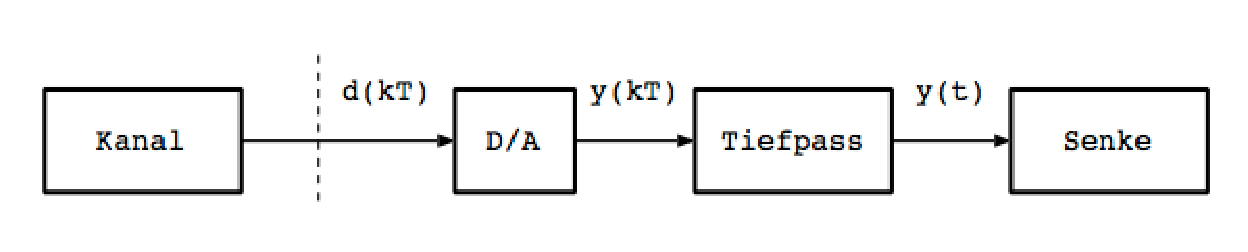
\includegraphics[scale=0.7, trim = 0cm 0cm 0cm 0cm, clip]{./Bilder/PCM_Decodierung}
            \caption{PCM Decodierung}
            \cite{PCM_Decodierung}
    \end{figure}
    
	
	Die PCM-Übertragung ist nur einer von vielen Verfahren der
	Digitalisierung, bei der eine Verringerung der notwendigen Bitrate möglich
	ist.Diese Übertragungsverfahren können mit dem Begriff Quellencodierung
	zusammengefasst werden und versichern keinen Qualitätsverlust. Um die besagte Bitrate zu verringern,
	werden die statistischen Eigenschaften der Nachrichtensignale und die
	Wahrnehmungseigenschaften der Menschen genutzt (Datenkompression).
	
	
	\end{quote}%section

%--------------------------------------------------------------------
%--------------------------------------------------------------------    
\section{Vorbereitungsaufgabe}
\begin{quote}
	
	Die theoretische Aufgabe für die Vorbereitung des Labortermin bestand darin,
	sich erneut mit dem Kapitel über Pulscodemodulation aus dem Skript zu
	beschäftigen. Das Wesentliche wurde in dem Theorieabschnitt des Protokolls
	erläutert. Außerdem sollten wir uns mit der Funktionsweise der für
	die PCM-Übertargungsstrecke relevanten Module des ETT-Schaltbretts vertraut
	machen und uns ein Blockschaltbild erarbeiten, welches den Aufbau realsieren
	könnte.\\
	
	Zuletzt sollte das in der Vorgabe gegebene MATLAB Skript PCM\_Analyse.m so
	vervollständigt werden, dass die Datei bei der Ausführung automatisch die
	PCM-Encoder-Kennlinie bestimmt. Der Code konnte anhand der Datei
	pcm\_data\_test.mat getestet und kontrolliert werden. \\
	
	Die erste Herausforderung war es den Anfang eines Bitwortes zu bestimmen. Dazu haben wir den Vektor Rahmen genommen,
	der auf dem letzten Bit eines Wortes ein High Pegel sendet. Diesen haben wir so um eine Stelle nach links
	verschoben und anschließend von sich selbst abgezogen, so dass er ausschließlich zu Beginn eines
	neuen Bitwortes eine $1$ sendet.\\
	Anschließend haben wir alle Bitwörter nacheinander bearbeitet und die Zahl der Abtastwerte und deren Wert den $8$ Bit
	eines jeden Bitwortes zugeordnet.
	Zum Schluss haben wir noch die binären Werte in Decimalwerte umgerechnet und den jeweiligen originalen Spannungswert
	aus den Messwerten bestimmt.\\
	Diese beiden Vektoren zueinander geplottet ergeben die PCM-Encoder-Kennlinie. Die Kennlinie selbst betrachten wir in
	der Auswertung genauer.
	
\end{quote}%Theorie beenden

%--------------------------------------------------------------------
%--------------------------------------------------------------------    

    
\section{Labordurchführung}
\begin{quote}

    \subsection{Aufgabe 2.1 - Bestimmen der PCM-Encoder-Kennlinie}
    \begin{quote}
         
         Bei diesem Aufgabenteil sollte die PCM-Encoder-Kennlinie des Quantisierers bestimmt werden, der in dem
         Steckbrett eingebaut ist. Dazu haben wir ähnlich wie bei der Vorbereitungsaufgabe ein Quellsignal und das
         dazugehörige Encodierte Signal abgespeichert.\\
         Als Signal sollten wir ein Dreieckssignal mit einer Aplitude von ein wenig über $4 V_{pp}$ verwenden. Diese
         Amplitude sollen wir wählen, da der eingebaute Quantisierer auf ein Spannungsbereich von $\pm 2 V$ ausgelegt
         ist, und wir diesen Bereich komplett ausnutzen wollen.\\
         Dieses Quellsignal lassen wir von dem PCM Encoder des Steckbretts modulieren. Dazu geben wir das Quellsignal
         auf den Eingang des PCM Encoders sowie ein $100 kHz$ Rechtecksignal auf den Taktgeber des Encoders. Die beiden
         Ausgänge PCM-Data sowie Framesynchonisation addieren wir und und greifen diesen Ausgang zum abspeichern ab.\\
         Damit das PCM-Signal später von dem Rahmen getrennt werden kann achten wir darauf, dass die Aplitude des PCM
         Signals $5 V$ beträgt und die Amplitude des Rahmensignals $8 V$. Auf diese Weise kann das Matlab Skript
         ``Split'' die beiden Signale voneinander trennen.
         
         Diese abgespeicherten Daten analysieren wir mit unserem in der Vorbereitungsaufgabe geschriebenen Matlab-Skript
         und errechnen uns die PCM-Kennlinie des Quentisierers. Die genaue Kennlinie ist in der Auswertung zu
         sehen.\vspace{1em}
         
         Der genau Aufbau sah folgendermaßen aus:
         \begin{figure}[H]
            \centering
                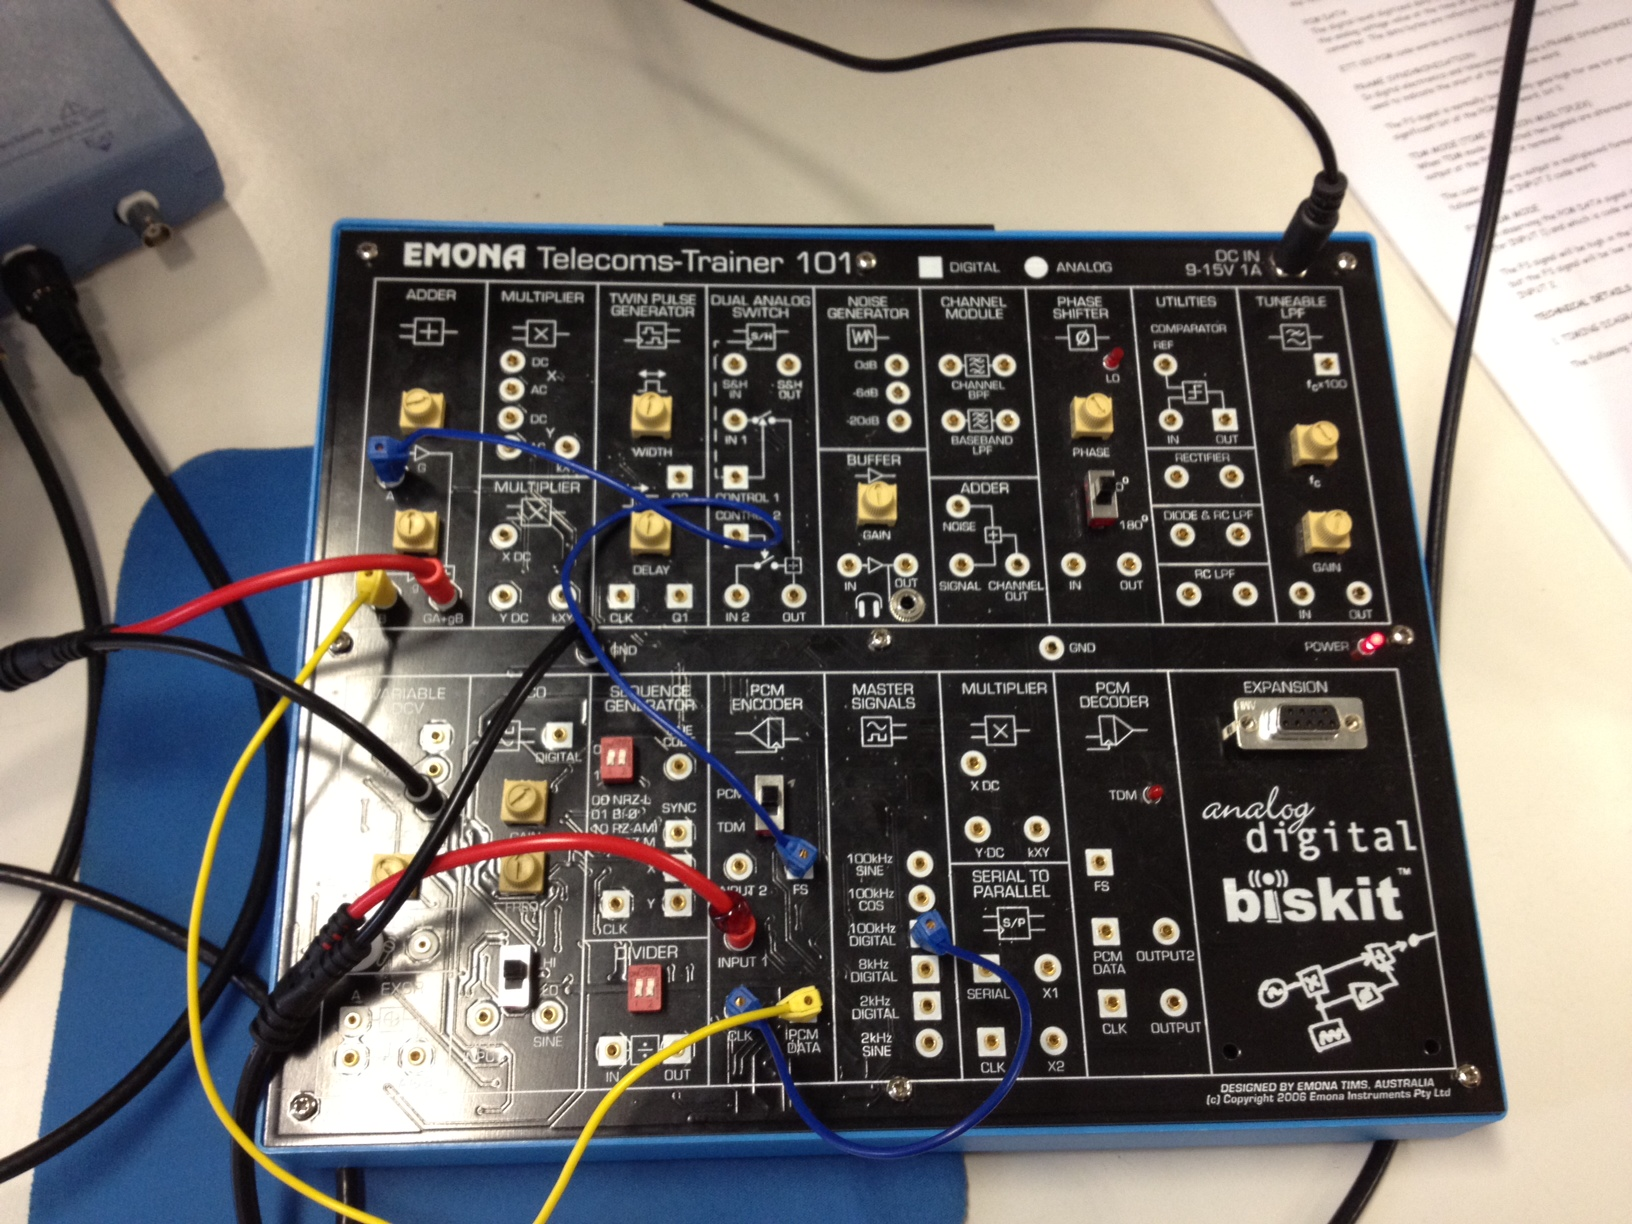
\includegraphics[scale=0.17, trim = 0cm 0cm 0cm 0cm,
                clip]{./Bilder/Aufgabe_2_1}
                    \caption{Aufbau Aufgabe 2.1}
            \end{figure}
    
         
    \end{quote}  % Ende Subsection PCM Encoder-Kennlinie
    
    \subsection{Aufgabe 2.2 - Quantisierungsfehler}
    \begin{quote}
       
       In der zweiten Aufgabe im Praktikum sollte der Quantisierungsfehler einer
       PCM-Übertragungsstrecke bestimmt werden. Dafür wurde zunächst die
       Einstellungen am Oszilloskop auf $5\frac{ms}{div}$ und auf $5ks$
       gestellt. Es wurde jeweils ein Sinusquellsignal und ein
       Dreieckquellsignal mit einer Clockfrequenz von $8kHz$ und $100kHz$ zuerst
       codiert und anschließend im Decoder des ETT decodiert und ohne
       rekonstruierenden Tiefpass mit dem Eingangssignal in den Vergleich
       gesetzt. Für Encoder und Decoder wurde für jede Messung die selbe
       Taktfrequenz verwendet. Außerdem führten die FS- und die PCM Data Signale
       des Encoders direkt in die entsprechenden Eingänge des Decoders. Der
       Aufbau ist auf diesem Bild nachvollziehbar:
       
       \begin{figure}[H]
            \centering
                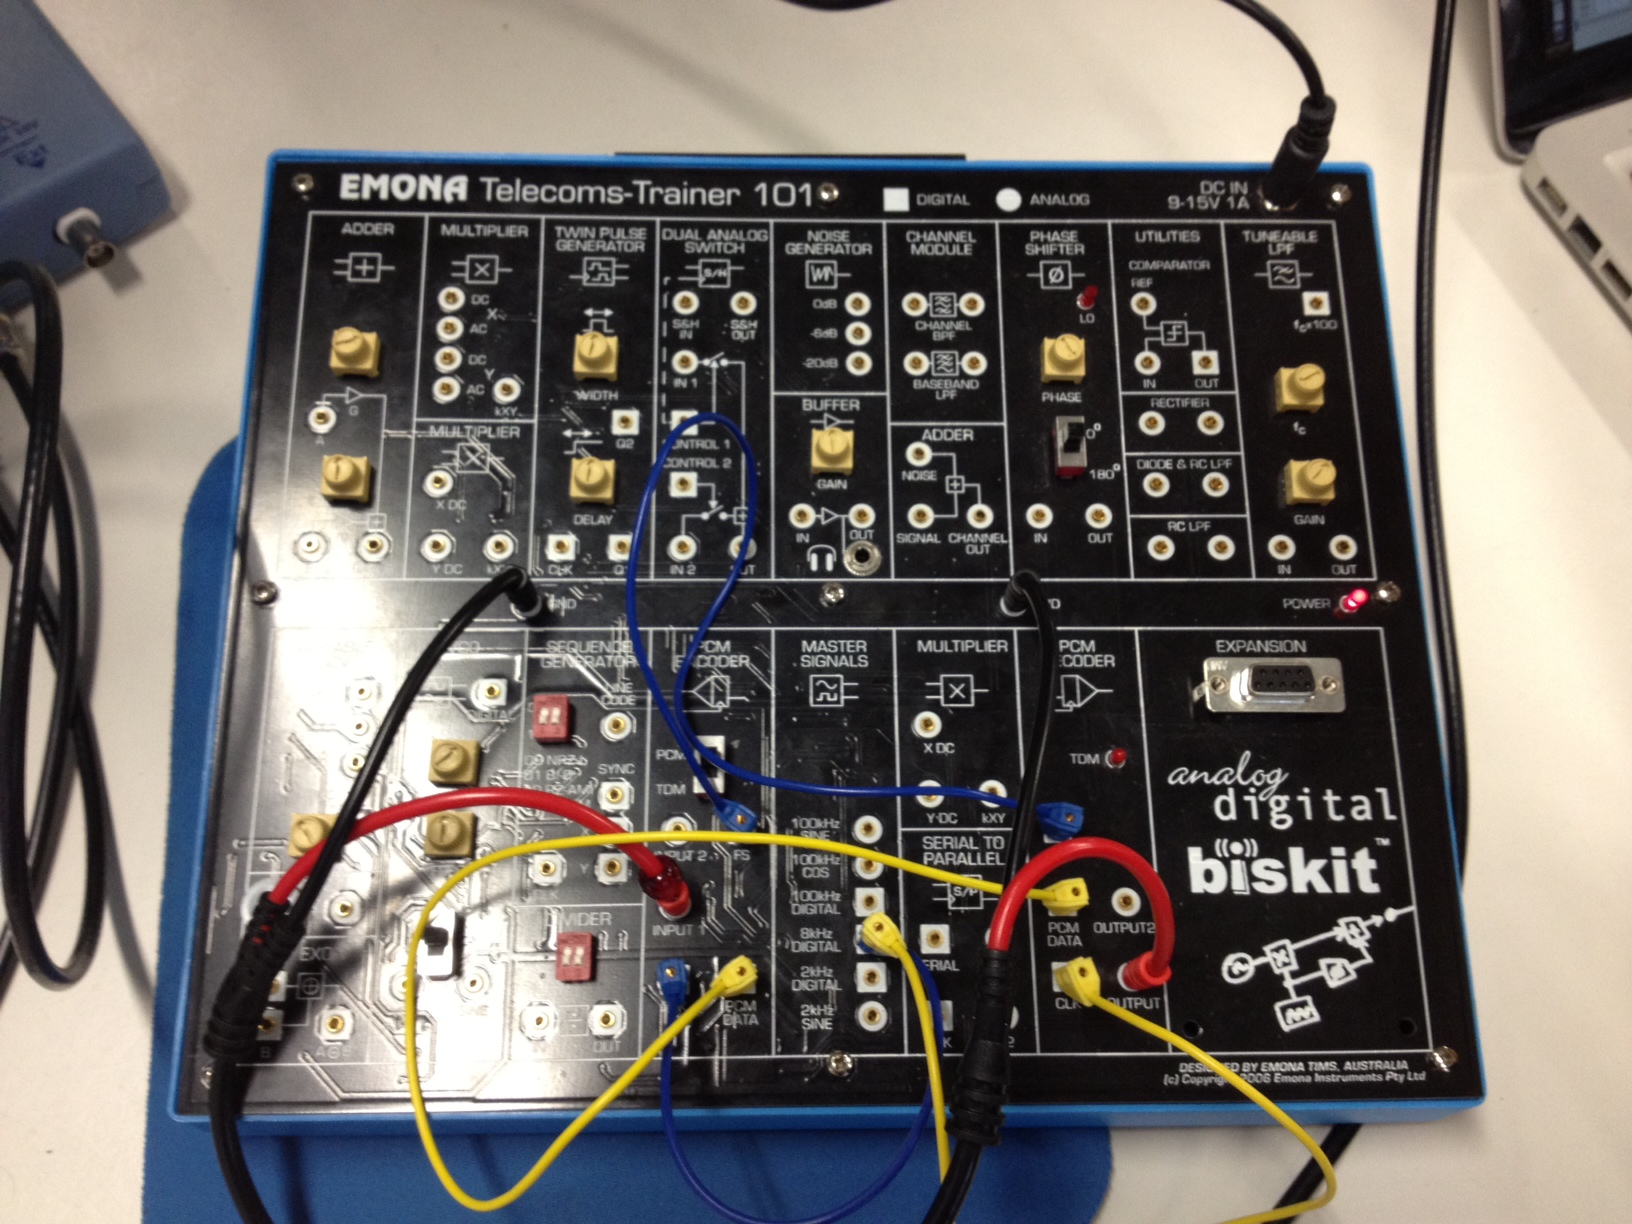
\includegraphics[scale=0.17, trim = 0cm 0cm 0cm 0cm,
                clip]{./Bilder/Aufgabe_2_2}
                    \caption{Aufbau Aufgabe 2.2}
       \end{figure}
       
       Mit den gemessenen Eingangs- und Ausgangssignalen konnte anhand der von
       uns erweiterten Datei Quantisierungsfehler.m der Quantisierungsfehler
       bestimmt und als Histogramm mit $10$ gleich großen Bins in
       einem Bereich von $\pm 0.3V$ dargestellt werden. Wichtig dabei war es,
       beide Signale zuerst mittelwertfrei und amplitudengleich zu richten.
       Außerdem musste mithilfe einer Kreuzkorrelation der zeitliche Verschub
       beider Signale ermittelt und kompensiert werden.\\
       
       Zuletzt wurde noch das Leistungsdichtespektrum (LDS) des
       Quantisierungsfehlers untersucht.
       
    \end{quote}  % Ende Subsection Quantisierungsfehler         

\end{quote}%beende Labordurchführung

%--------------------------------------------------------------------
%--------------------------------------------------------------------    

    
\section{Auswertung}
\begin{quote}
    
    \subsection{Vorbereitungsaufgabe}
    \begin{quote}
        Nun betrachten wir die in der Vorbereitungsaufgabe ermittelte PCM-Encoder-Kennlinie.
        
        \begin{figure}[H]
        \centering
        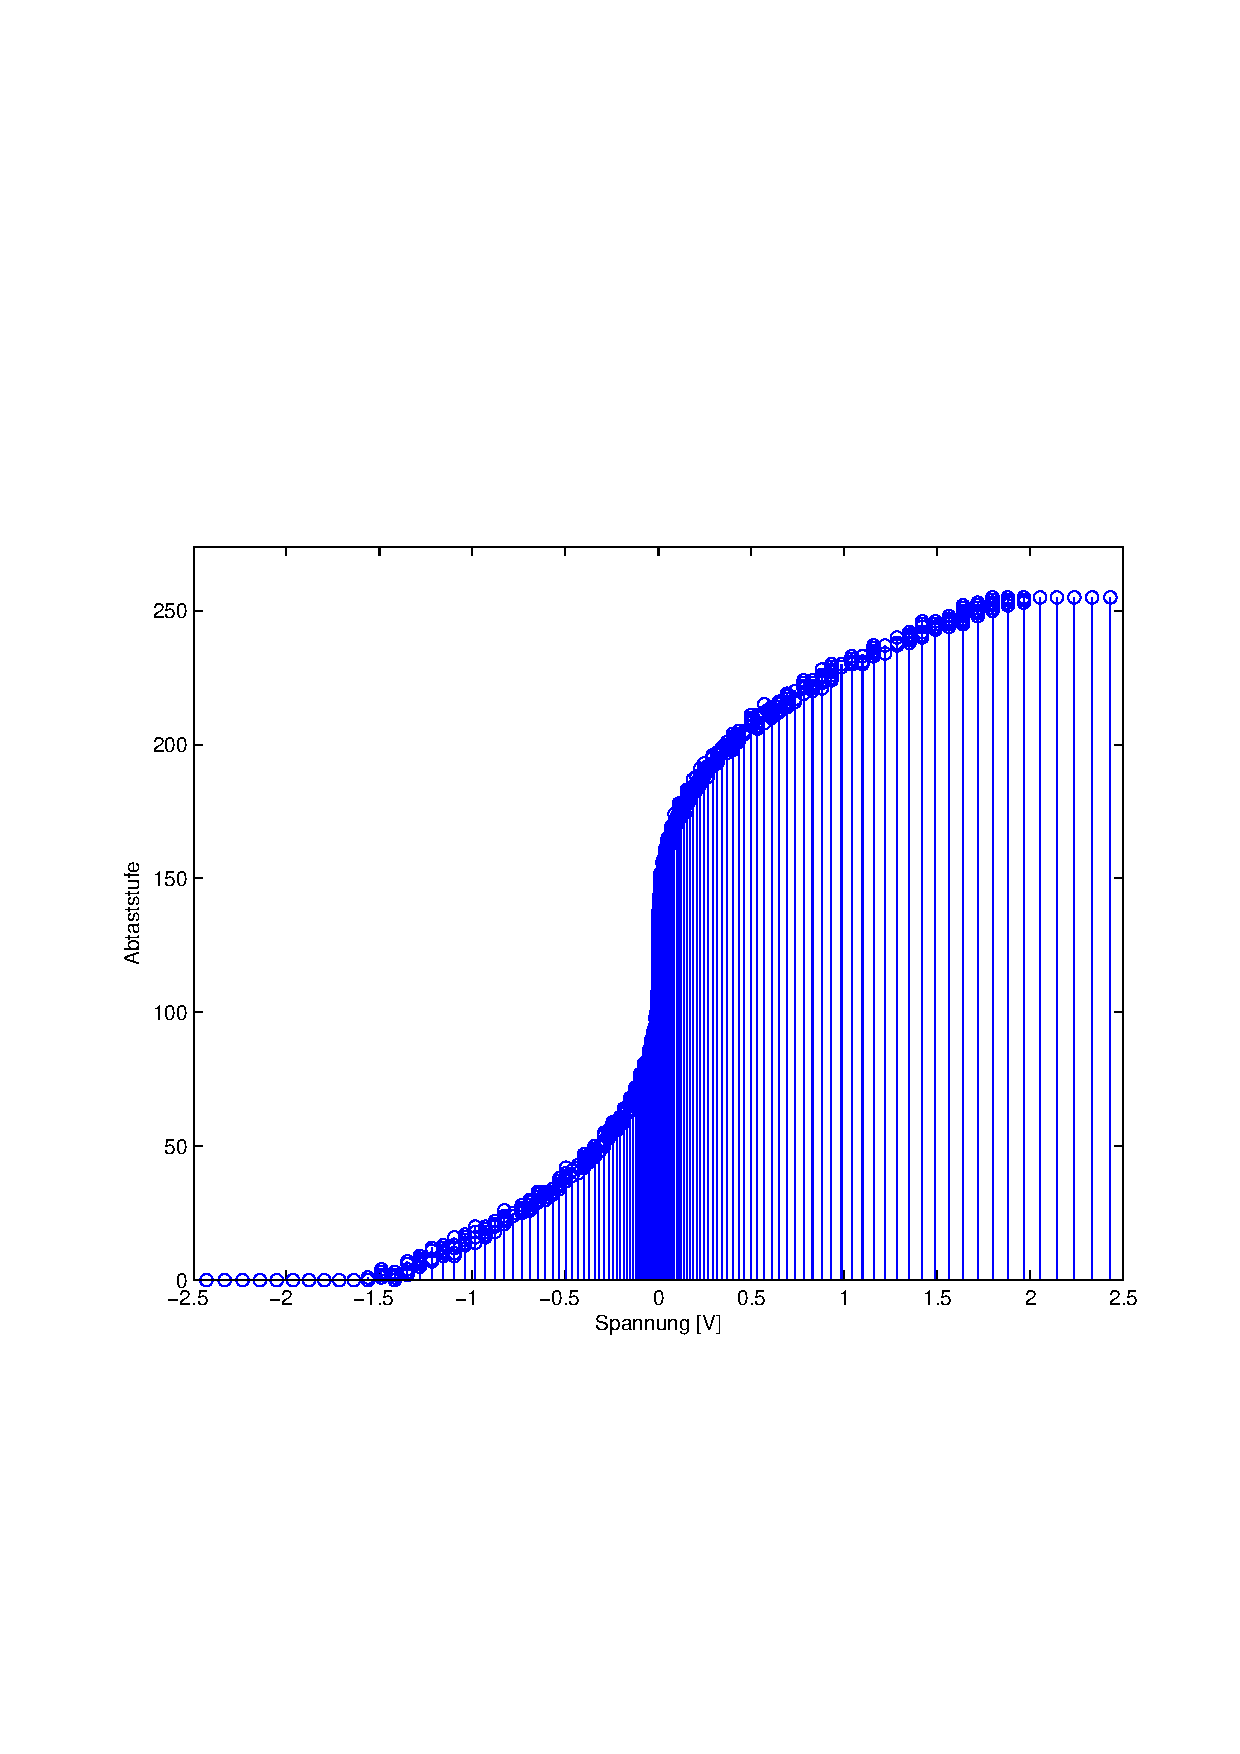
\includegraphics[scale=0.7, trim = 2cm 7cm 1cm 9cm, clip]{./Bilder/Kennlinie_Vorbereitungsaufgabe}
            \caption{PCM-Encoder-Kennlinie Vorbereitungsaufgabe}
        \end{figure}
        
        Es fällt auf, dass es sich bei dieser Kennlinie um eine nichtlinieare Kennlinie handlet. Der Spannungsbereich um
        $0V$ ist wesentlich höher aufgelöst als an den Rändern der Kennlinie. Mit anderen Worten, die
        Quantisierungsstufen liegen um $0V$ dichter beieinander als bei $\pm 1.5V$.\vspace{1em}
        
        Ein solcher Quantisierer kann interessant sein wenn es einen besondern Bereich innerhalb des Nutzsignals gibt,
        der mit höherer Auflösung übertragen werden soll als andere. Als Konsequenz verschlechtert sich dadurch
        automatisch die Auflösung des randbereichs, da ja nicht mehr Bits bzw. Stufen zur verfügung
        stehen. Als Konsequenz wird der Quantisierungsfehler im hochaufgelösten Bereich kleiner und beim
        niedrig Aufgelösten Bereich größer als bei gleichverteilten Quantisierungsstufen.\vspace{1em}
        
        Weiter lässt sich bei der Kennlinie beobachten, dass sowohl am unteren als auch am oberen Bereich der
        Kennlinie die Messwerte abflachen und auf dem Wert $0$ bzw. $255$ bleiben. In beiden Fällen gerät der
        Quantisierer in die Sättigung und sendet den minimalen bzw. den maximal möglichen Wert.\\
        Auffallend ist, dass die Grenzen für die der Quantisierer in Sättigung geht nicht symmetrisch sind. Im unteren
        Bereich geht der Quantisierer schon für $-1,6 V$ in Sättigung während er im oberen Bereich für $2 V$ in
        Sättigung geht.\\
        Die Ursache dafür vermuten wir in dem Quantisierer, der nunmal nicht ideal arbeitet sondern eben real umgesetzt
        ist.\vspace{1em}
        
        Außerdem lassen sich mehrere Stufen für einen Spannungswert ausmachen. Diese Stufen liegen jedoch sehr dicht
        beieinander. Die Ursache dafür wird sein, dass mehrmals der selbe Spannungswert im Originalsignal vorkam und
        ihm beim quantisieren unterschiedliche Wert zugeweisen wurden. Da diese Werte sich nur um max $4$ Stufen
        unterscheidet und diese Stufen sehr klein sind entsteht dadurch kein schwerwiegender Fehler. Jedoch wird es den
        Quantisierungsfehler verstärken. Denkbar ist auch, dass einzelne Bits während der Übertragung verfälscht
        wurden.\vspace{1em}
        
        Wenn man die Grafik bei dem Spannungswert $0V$ vergrößert fällt auf, dass die Kennlinie auch für diese Spannung
        einen Wert besitzt. Dadurch lässt sich darauf schließen, dass es sich bei dem eingesetzten Quantisierer um
        einen Midtread Quantisierer gehandelt hat. Im Falle eine Midrise Quantisierers hätte die Kennlinie
        zwei Stufen nahe bei der Spannung $0V$ jedoch keine genau bei diesem Spannungswert.
        
        
    
    \end{quote}  % Ende Subsection Vorbereitungsaufgabe
    
    \subsection{Aufgabe 2.1 - Bestimmen der PCM-Encoder-Kennlinie}
    \begin{quote}
        
        Als nächstes betrachten wir die PCM-Encoder-Kennlinie, die wir aus der Messung in Aufgabe $2.1$ ermittelt haben.
        
        \begin{figure}[H]
        \centering
            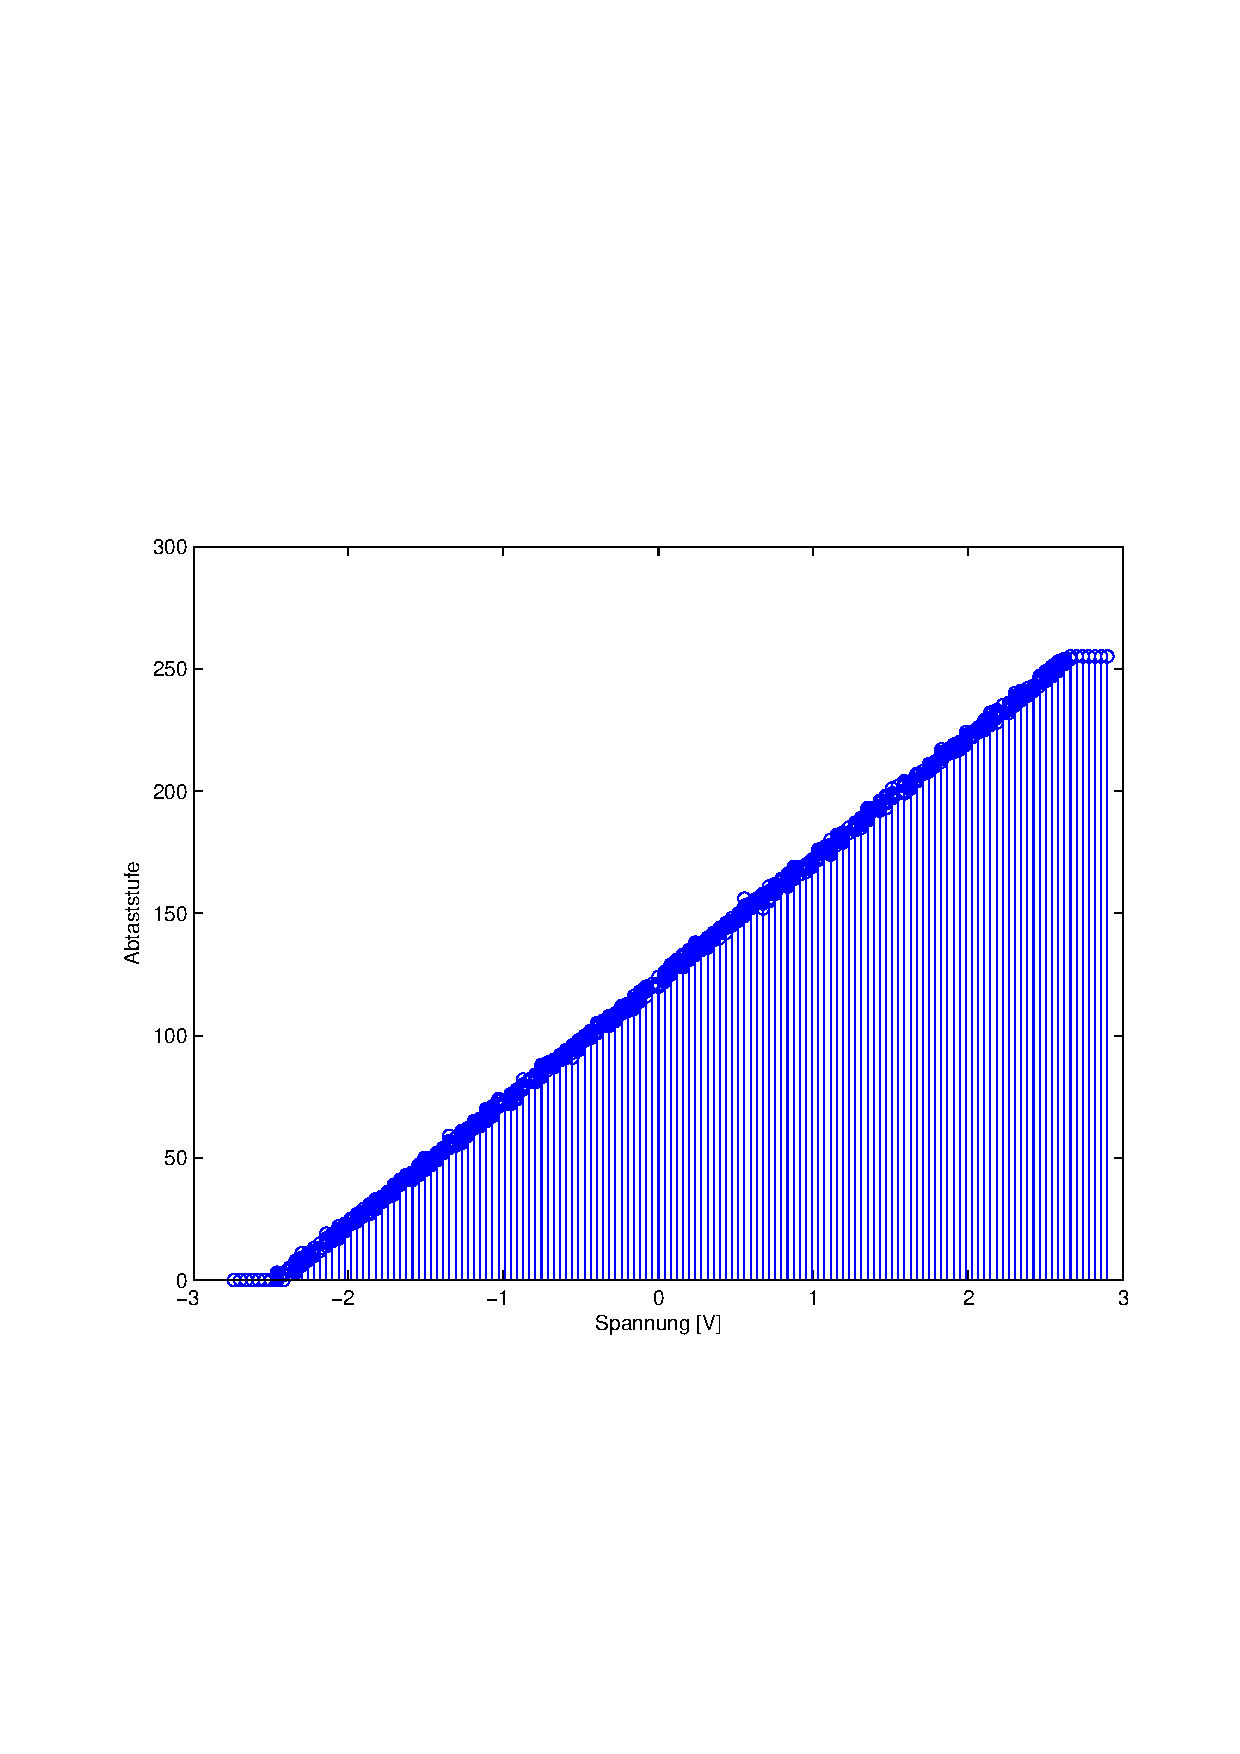
\includegraphics[scale=0.7, trim = 2cm 7cm 1cm 9cm, clip]{./Bilder/Kennlinie_Aufgabe_2_1}
                \caption{PCM-Encoder-Kennlinie Steckbrett}
        \end{figure}
        
        Diese PCM-Encoder-Kennlinie unterscheidet sich auffällig von der aus der Vorbereitungsaufgabe.
        Sie ist offensichtlich linear und die Abstände zwischen den Quantisierungsstufen sind gleich groß. Im Gegensatz
        zu dem Quantisierer in der Vorbereitungsaufgabe haben die Quantisierungsstufen in diesem Fall alle den selben
        Abstand. Daraus lässt sich herleiten, dass es sich um einen anderen Quantisier handelt als in der
        Vorbereitungsaufgabe.\vspace{1em}
        
        Bei der Bessung haben wir bewusst den maximalen Bereich des Quantisierers angesteuert. Auch das lässt sich in
        der Kennlinie Erkennen. Wie in der Vorbereitungsaufgabe geht der Quanisierer sowohl für sehr hohe Werte als auch
        für niedrige Werte in die Sättigung. Jedoch ist auch diese nicht symetrisch verteilt. Die untere
        Sättigungsgrenze liegt bei $-2,4 V$ und die obere bei $2,6 V$. Auch in diesem Fall vermuten wir die Ursache in
        dem realen Bauteil.\vspace{1em}
        
        Genau wie bei der Vorbereitungsaufgabe lassen sich auch bei dieser Kennlinie mehrere Abtaststufen für eine
        Spannungswert erkennen, die auf das selbe Phänomen zurückzuführen sind wie in der Vorbereitung.\\
        Da sich auch hier eine Stufe bei $0 V$ erkenne lässt handelt es sich auch diesesmal um einen Midtread
        Quantisierer.\vspace{1em}
        
        
    \end{quote}  % Ende Subsection PCM Encoder-Kennlinie
    
    \subsection{Aufgabe 2.2 - Quantisierungsfehler}
    \begin{quote}
    
        \subsubsection{Quantisierungsfehler und Histogramm}
        \begin{quote}
    
            Die Ergebnisse der Messung aus Aufgabe 2 ergaben für das Sinussignal mit
            einer Clockfrequenz von $8 kHz$ folgende Plots. Zuerst werden die
            mittelwertfreien Sende- und Empfangssignale bezüglich Amplitude und
            Zeitverschiebung aufeinander angepasst. Danach wird der
            Quantisierungsfehler und dessen Histogramm gebildet:
            
            \begin{center}
                \begin{tabular}{ll}
                
                \hspace{-4cm}
                    \begin{minipage}{0.6\textwidth}
                        \begin{figure}[H]
                            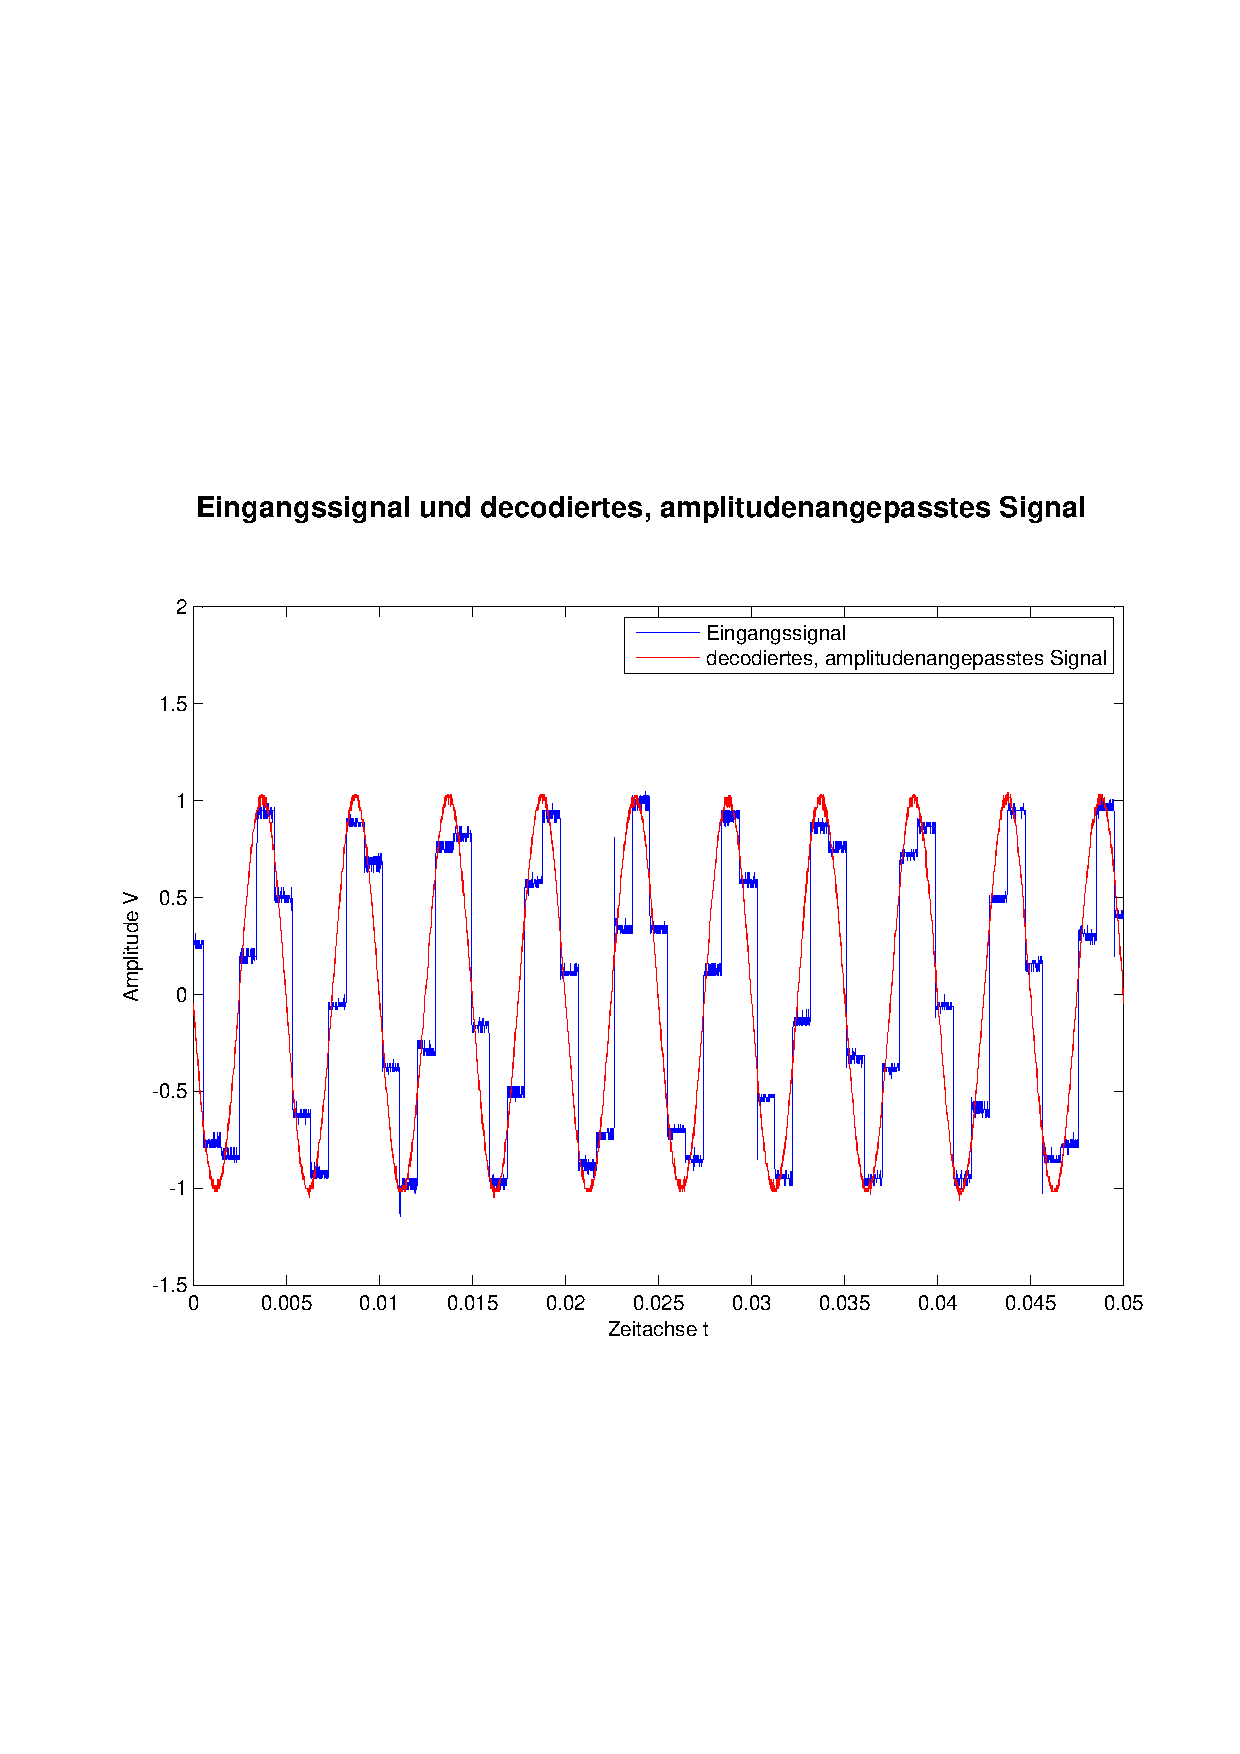
\includegraphics[scale=0.4, trim = 0.8cm 7cm 0.8cm
                            7.5cm, clip]
                            {./Bilder/sin8_Eingang_vs_DecodiertAmpl-angepasst}
                              \caption{Eingangssignal und decodiert, \newline
                              amplitudenangepasstes Signal}
                        \end{figure}
                    \end{minipage}
                    
                    \begin{minipage}{0.6\textwidth}
                        \begin{figure}[H]
                            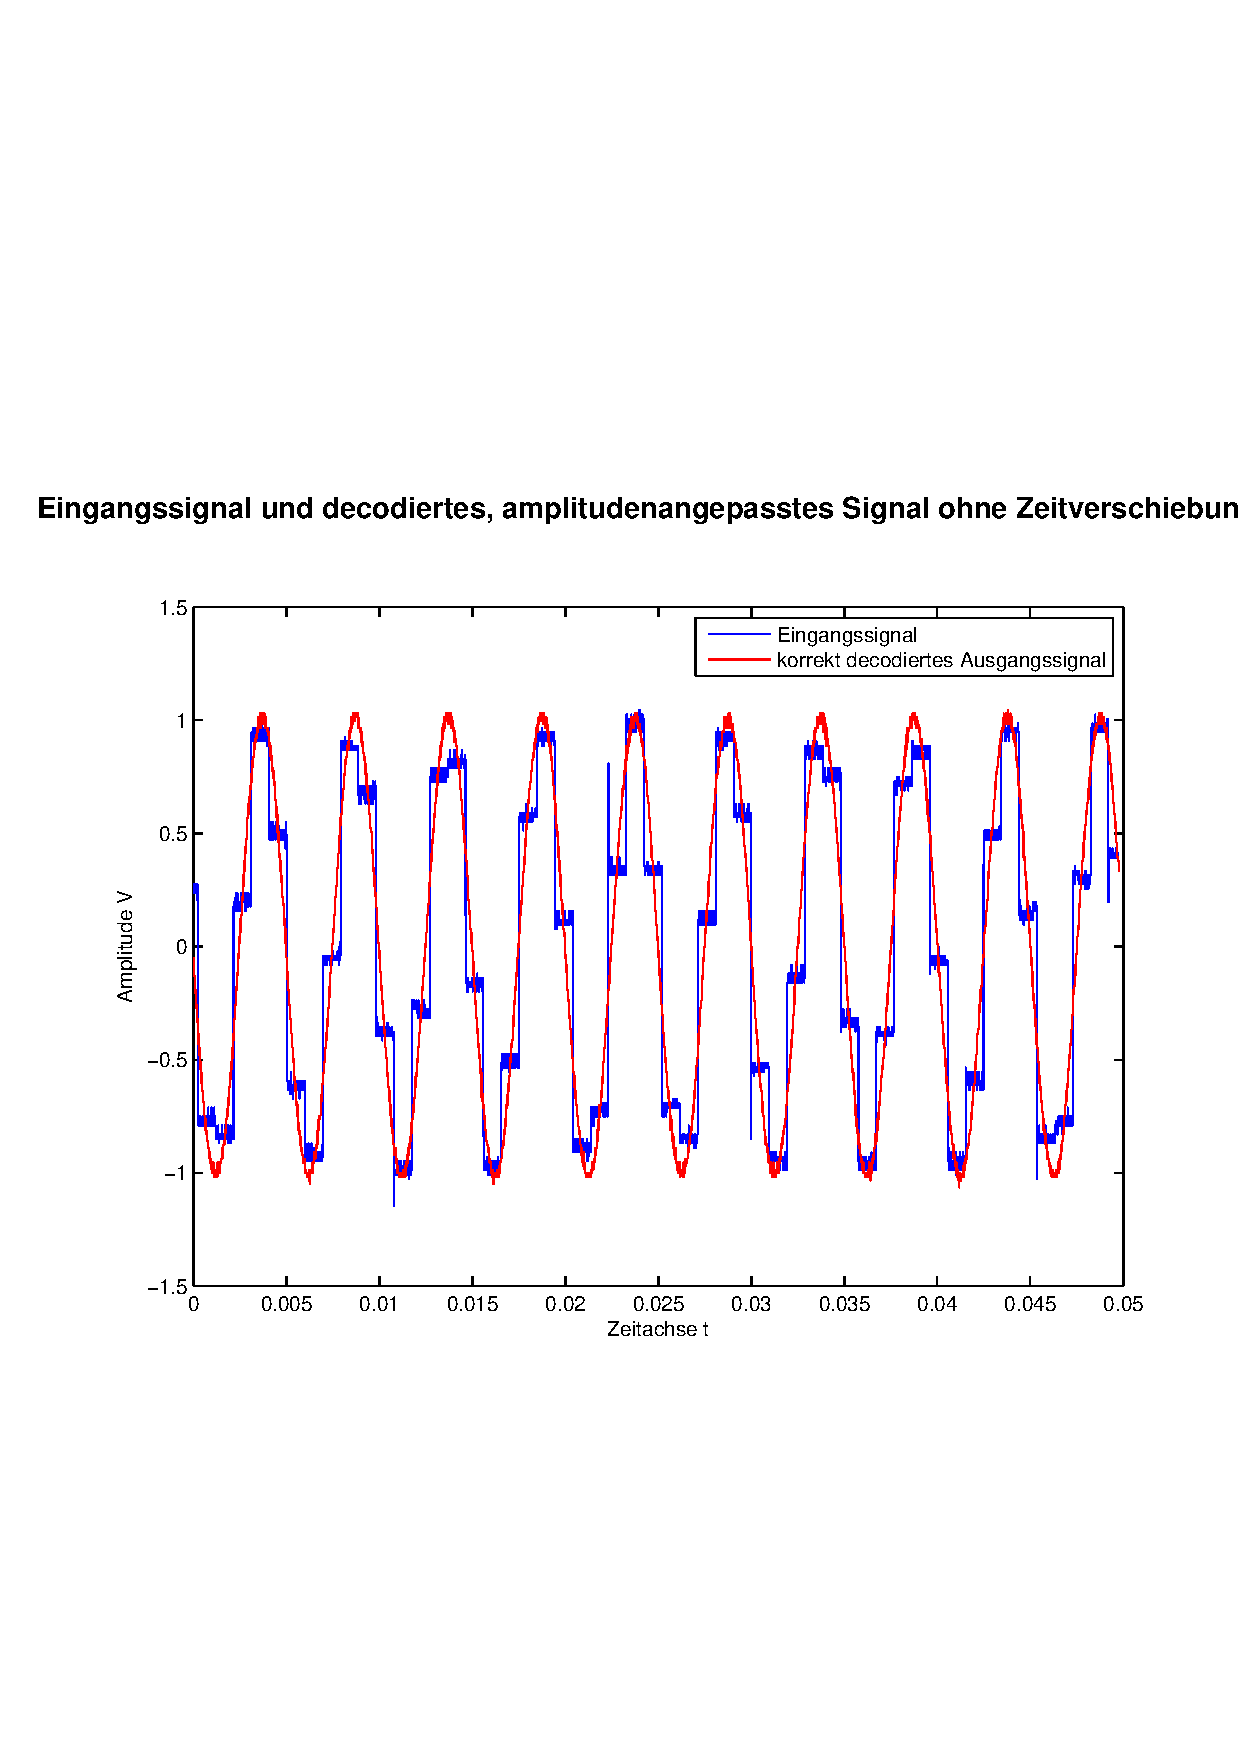
\includegraphics[scale=0.4,trim = 0cm 7cm 0cm
                            7.5cm, clip]
                            {./Bilder/sin8_Eingang_vs_korrektDecodiert}
                              \caption{Eingangssignal und
                              korrekt decodiertes Ausgangssignal}
                        \end{figure}
                    \end{minipage}
                
                \end{tabular}
            \end{center}
            
            \begin{center}
                \begin{tabular}{ll}
                
                \hspace{-4cm}
                    
                    \begin{minipage}{0.55\textwidth}
                        \begin{figure}[H]
                            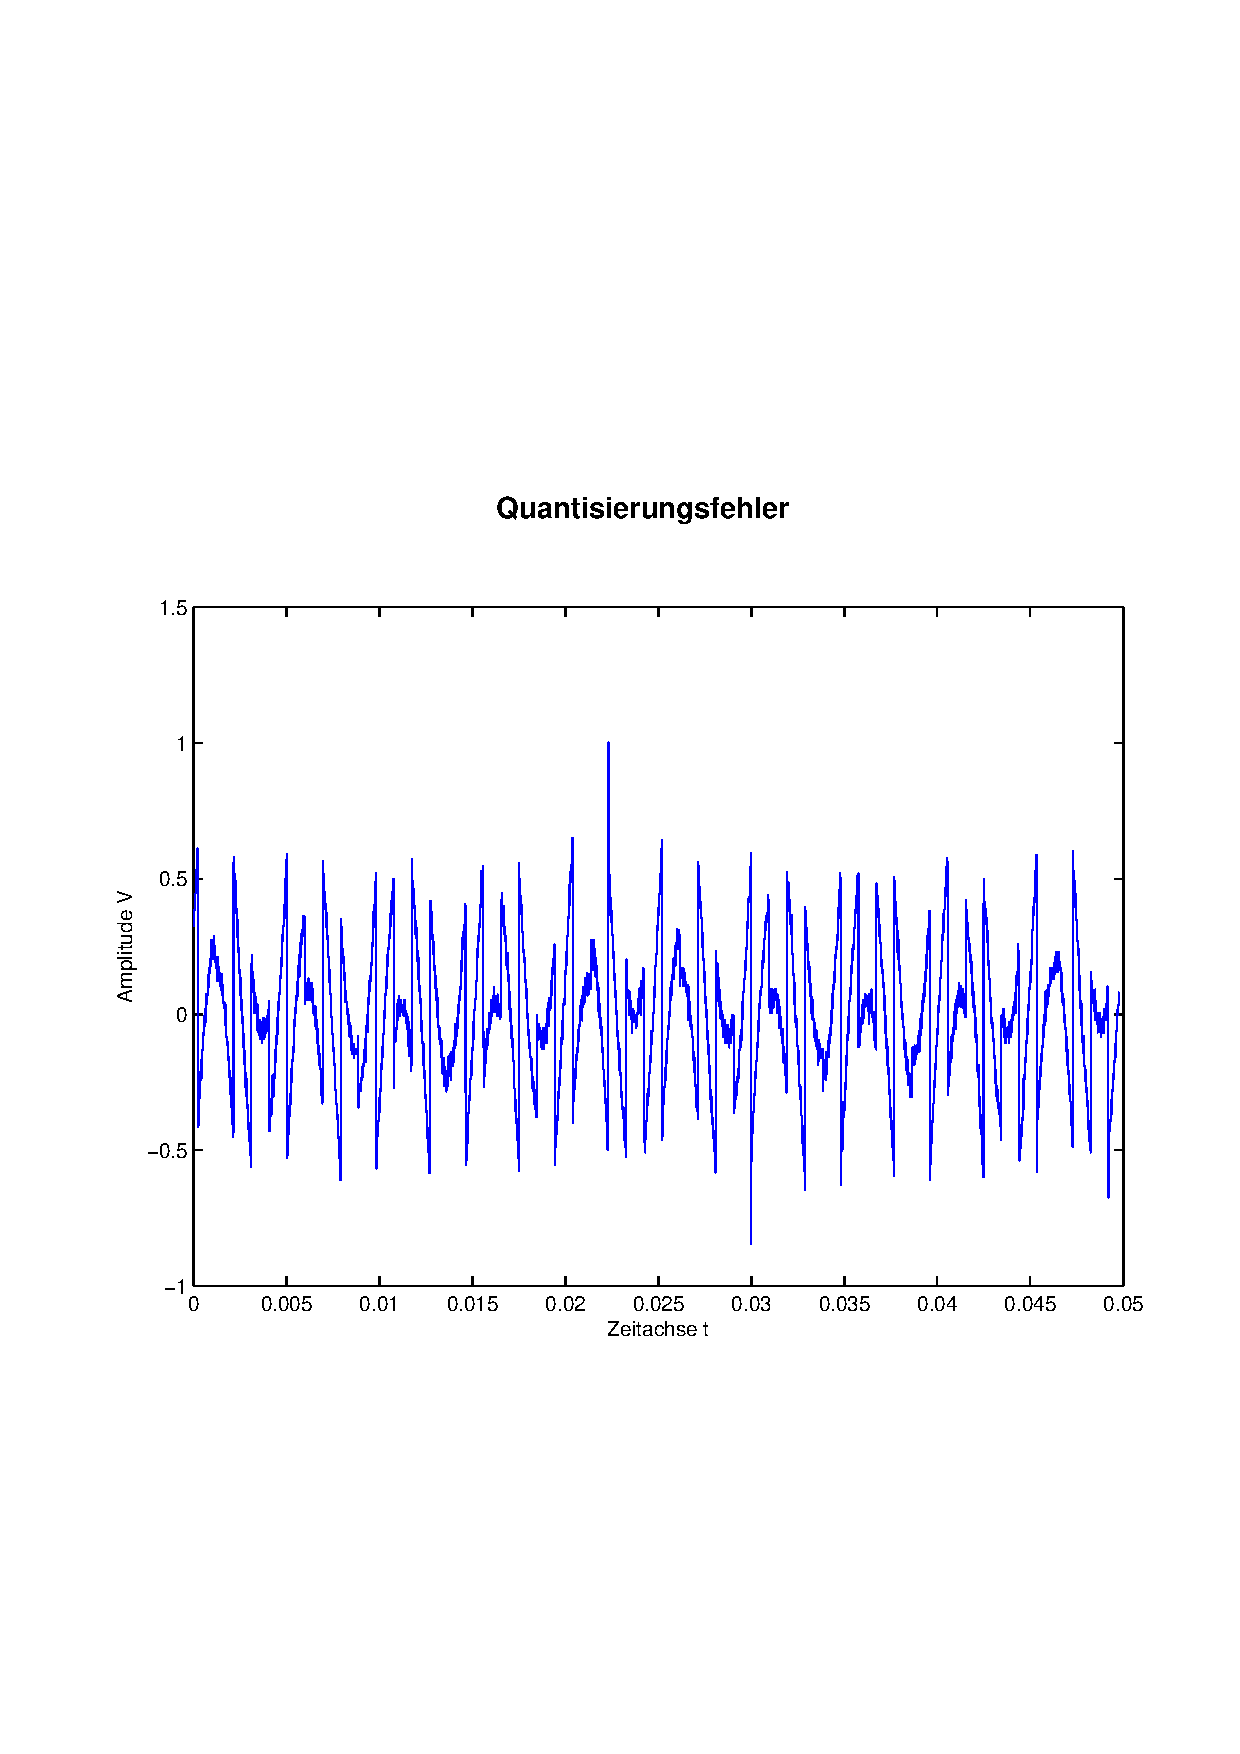
\includegraphics[scale=0.4, trim = 0cm 7cm 0cm
                            7.5cm, clip]
                            {./Bilder/sin8_Quantisierungsfehler}
                              \caption{Quntisierungsfehler (Sinus, 100kHz clk)}
                        \end{figure}
                    \end{minipage}
                                  
                    \begin{minipage}{0.6\textwidth}
                        \begin{figure}[H]
                            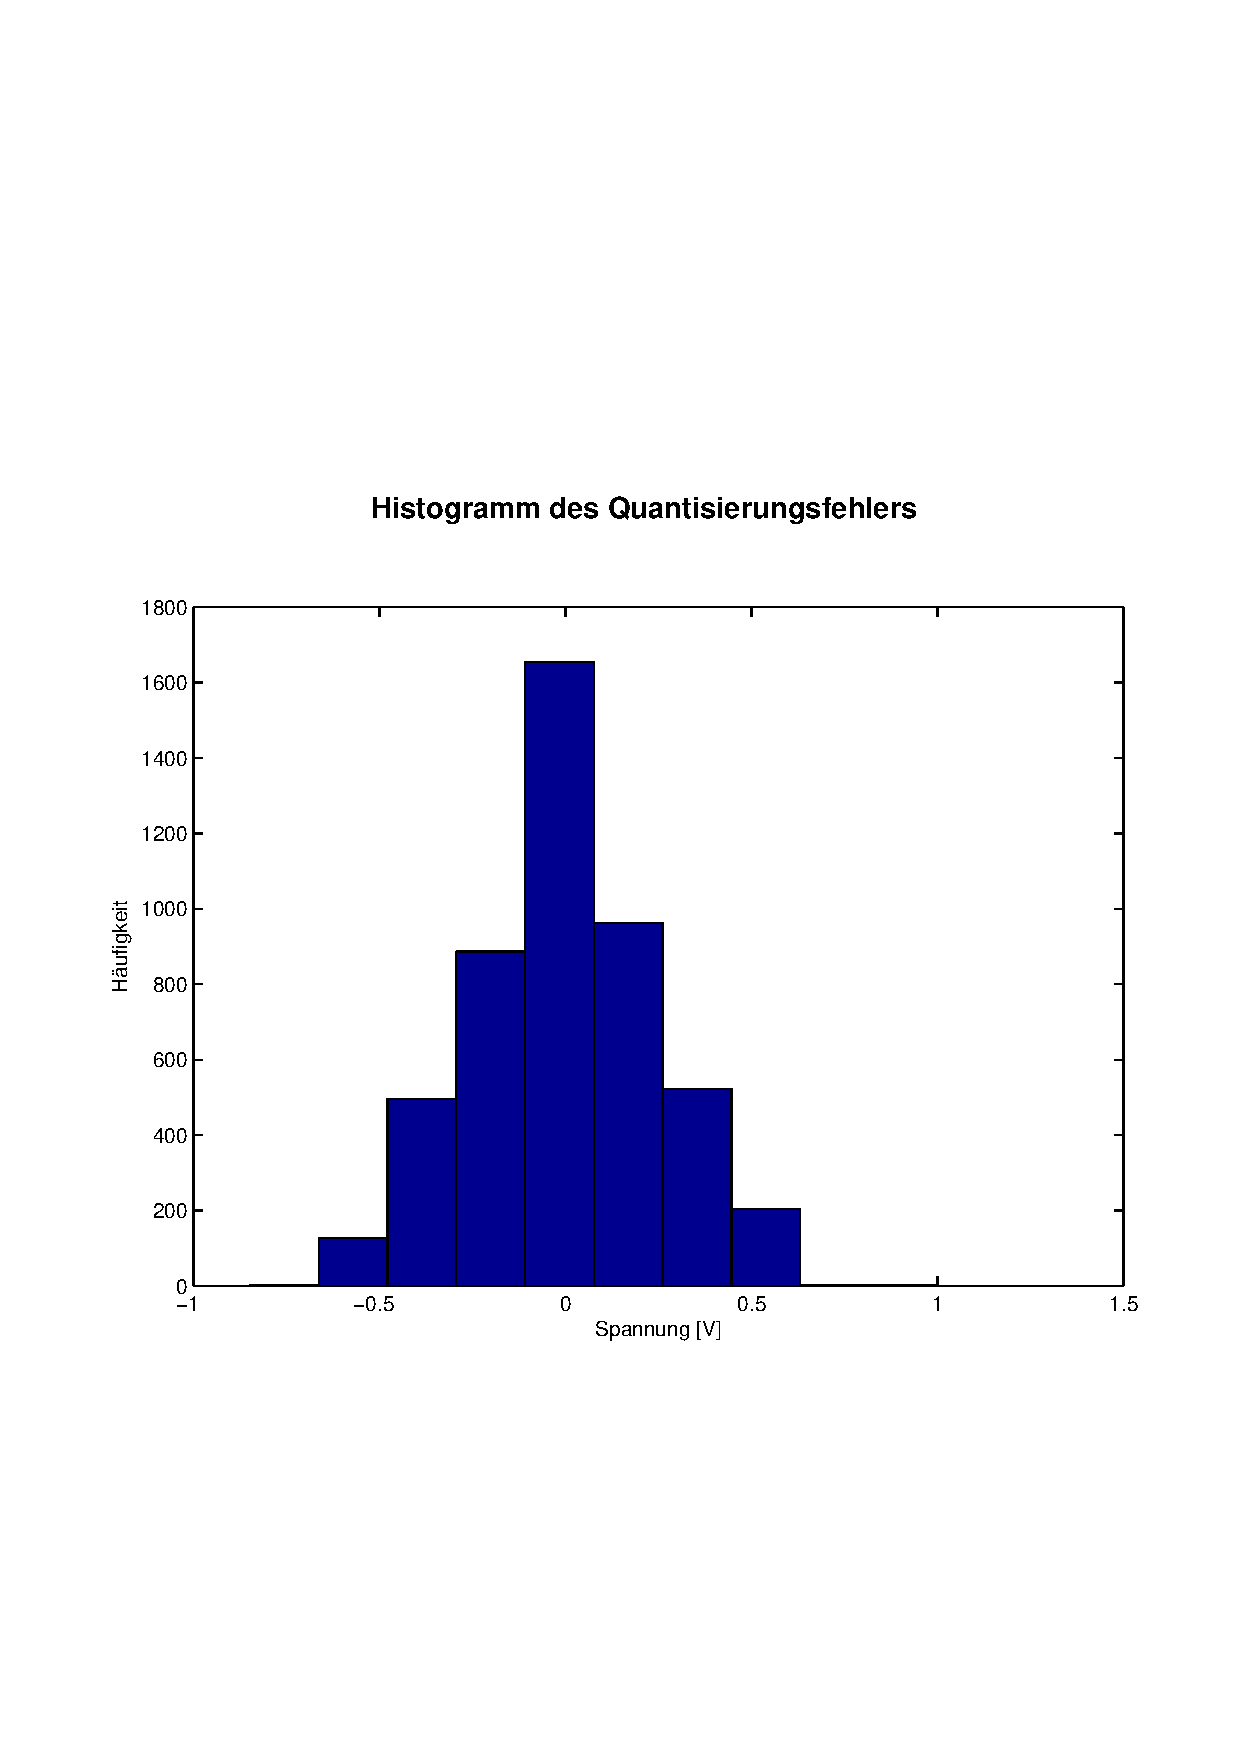
\includegraphics[scale=0.4, trim = 0cm 7cm 0cm
                            7.5cm, clip]
                            {./Bilder/sin8_Histogramm}
                              \caption{Histogramm des Quantisierungsfehlers}
                        \end{figure}
                    \end{minipage}
                
                \end{tabular}
            \end{center}
            \vspace{1em}
            
            \TODO{Plots erklären, was zum Quantisierungsfehler sagen}\\
            
            
            
            \vspace{1em}
            
            Als nächstes betrachten wir das selbe Sinussignal bei einer Abtastfrequenz von $100 kHz$. 
    
            \begin{center}
                \begin{tabular}{ll}
                
                \hspace{-4cm}
                    \begin{minipage}{0.6\textwidth}
                        \begin{figure}[H]
                            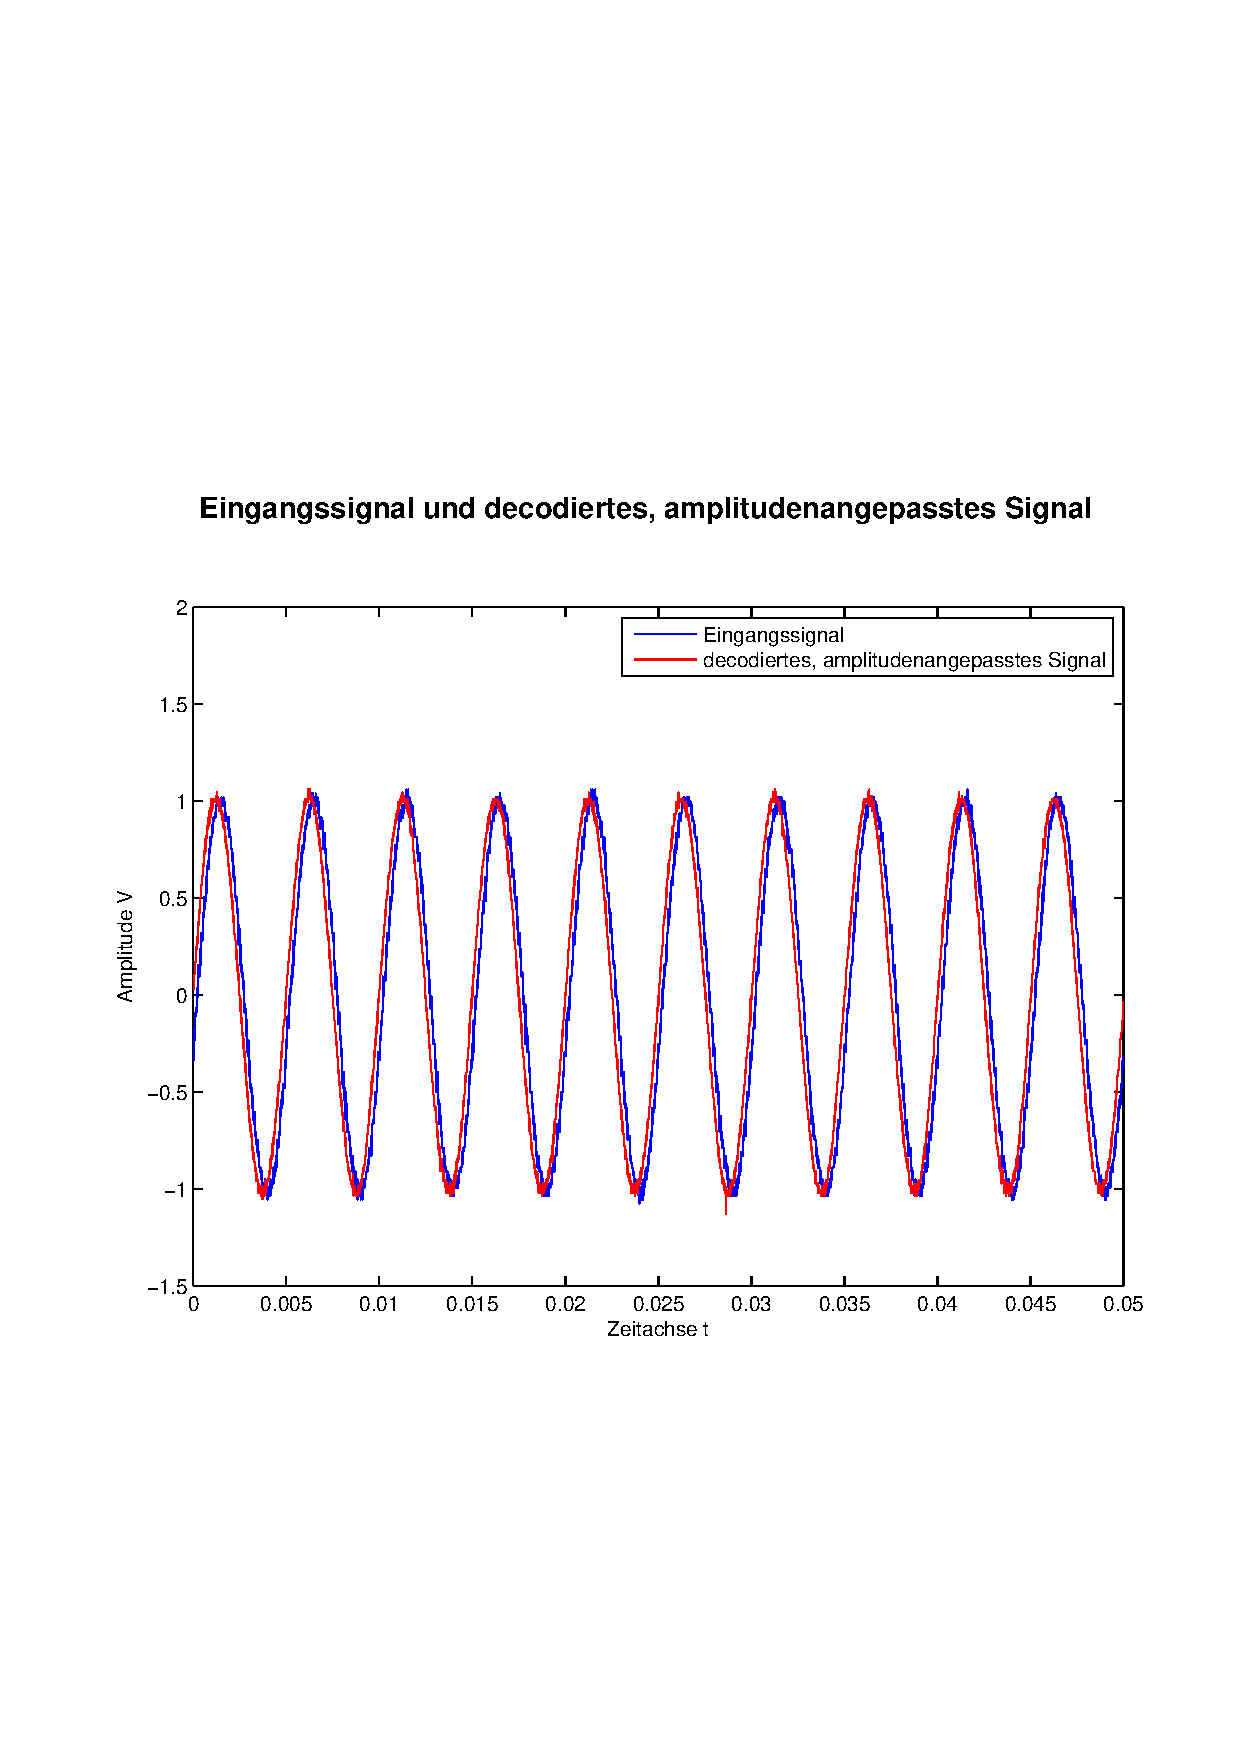
\includegraphics[scale=0.4, trim = 0.8cm 7cm 0.8cm
                            7.5cm, clip]
                            {./Bilder/sin100_Eingang_vs_DecodiertAmpl-angepasst}
                              \caption{Eingangssignal und decodiert, \newline
                              amplitudenangepasstes Signal}
                        \end{figure}
                    \end{minipage}
                    
                    \begin{minipage}{0.6\textwidth}
                        \begin{figure}[H]
                            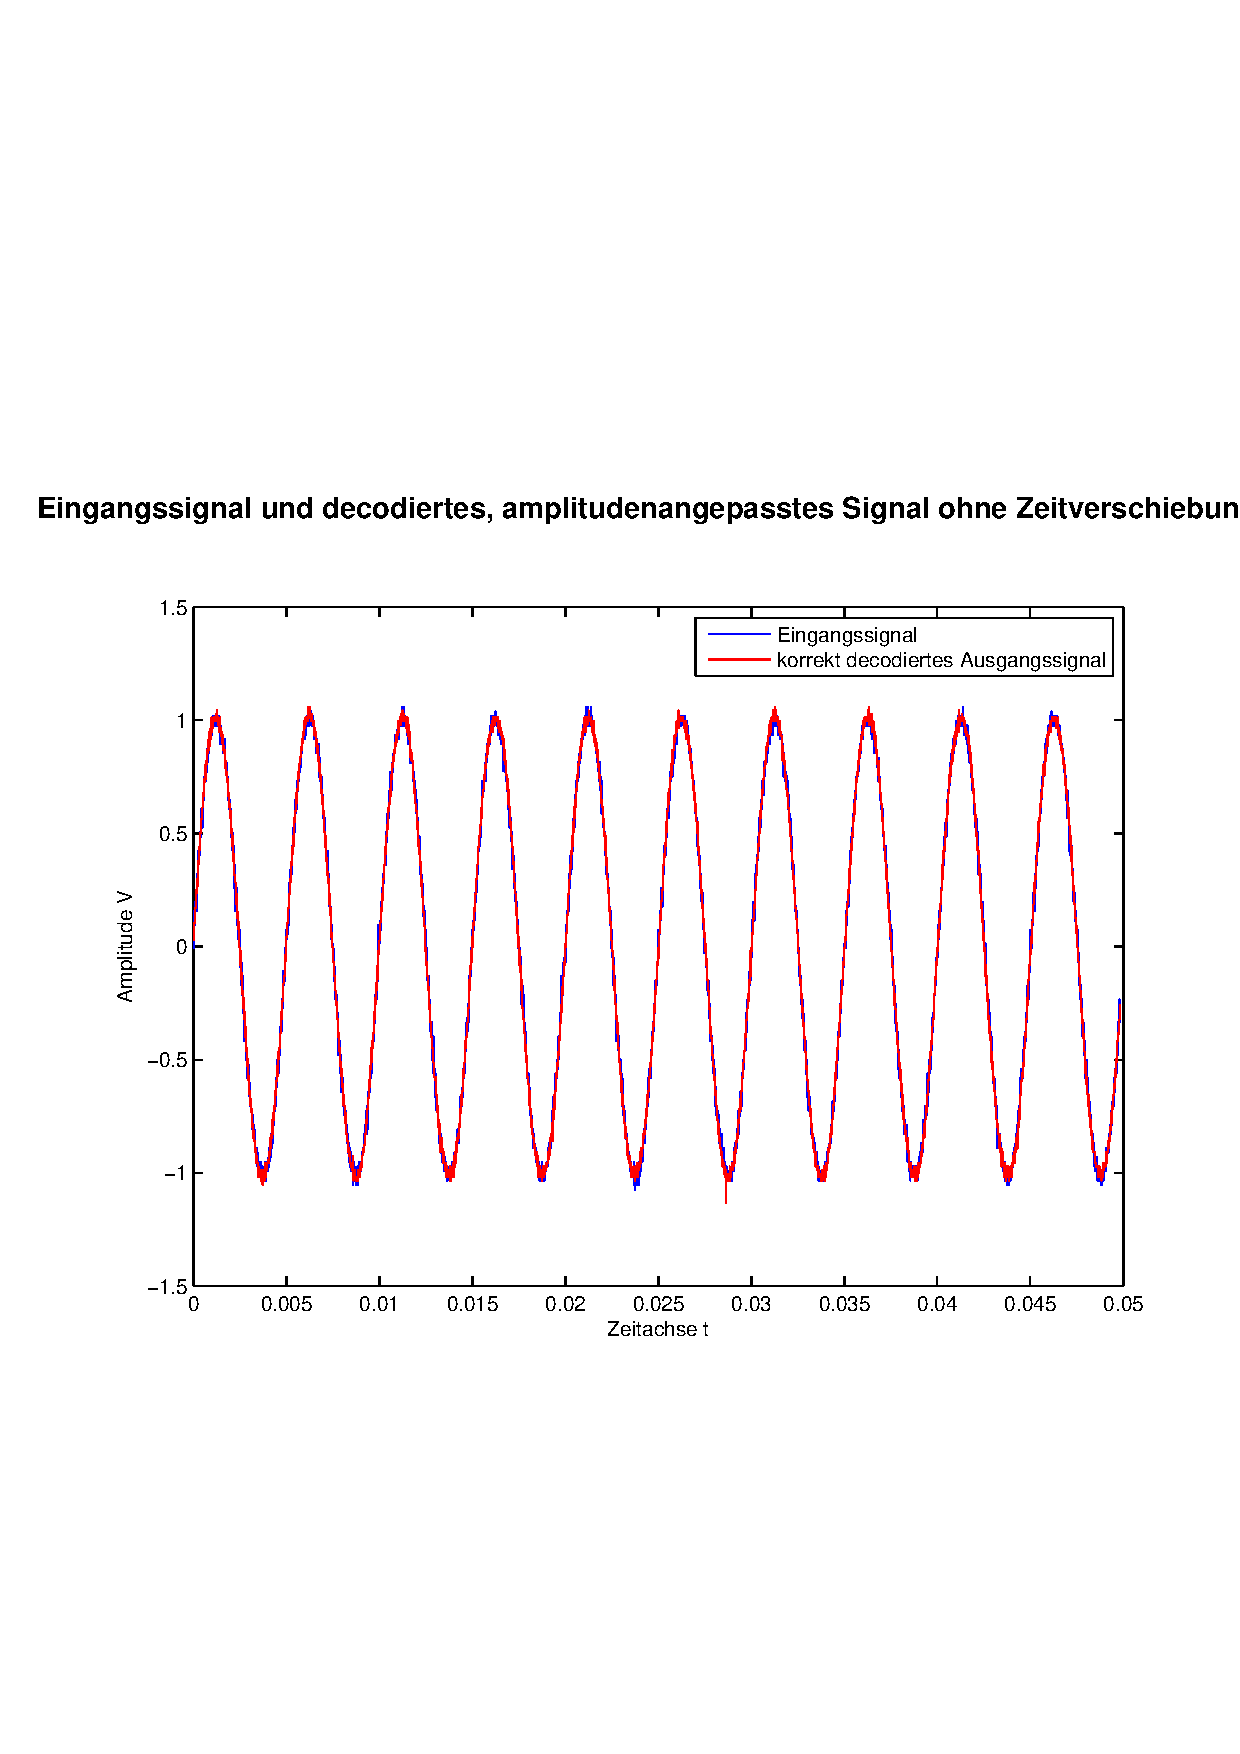
\includegraphics[scale=0.4,trim = 0cm 7cm 0cm
                            7.5cm, clip]
                            {./Bilder/sin100_Eingang_vs_korrektDecodiert}
                              \caption{Eingangssignal und korrekt decodiertes
                              Ausgangssignal}
                        \end{figure}
                    \end{minipage}
                
                \end{tabular}
            \end{center}
            
            
            
            \begin{center}
                \begin{tabular}{ll}
                
                \hspace{-4cm}
                    
                    \begin{minipage}{0.55\textwidth}
                        \begin{figure}[H]
                            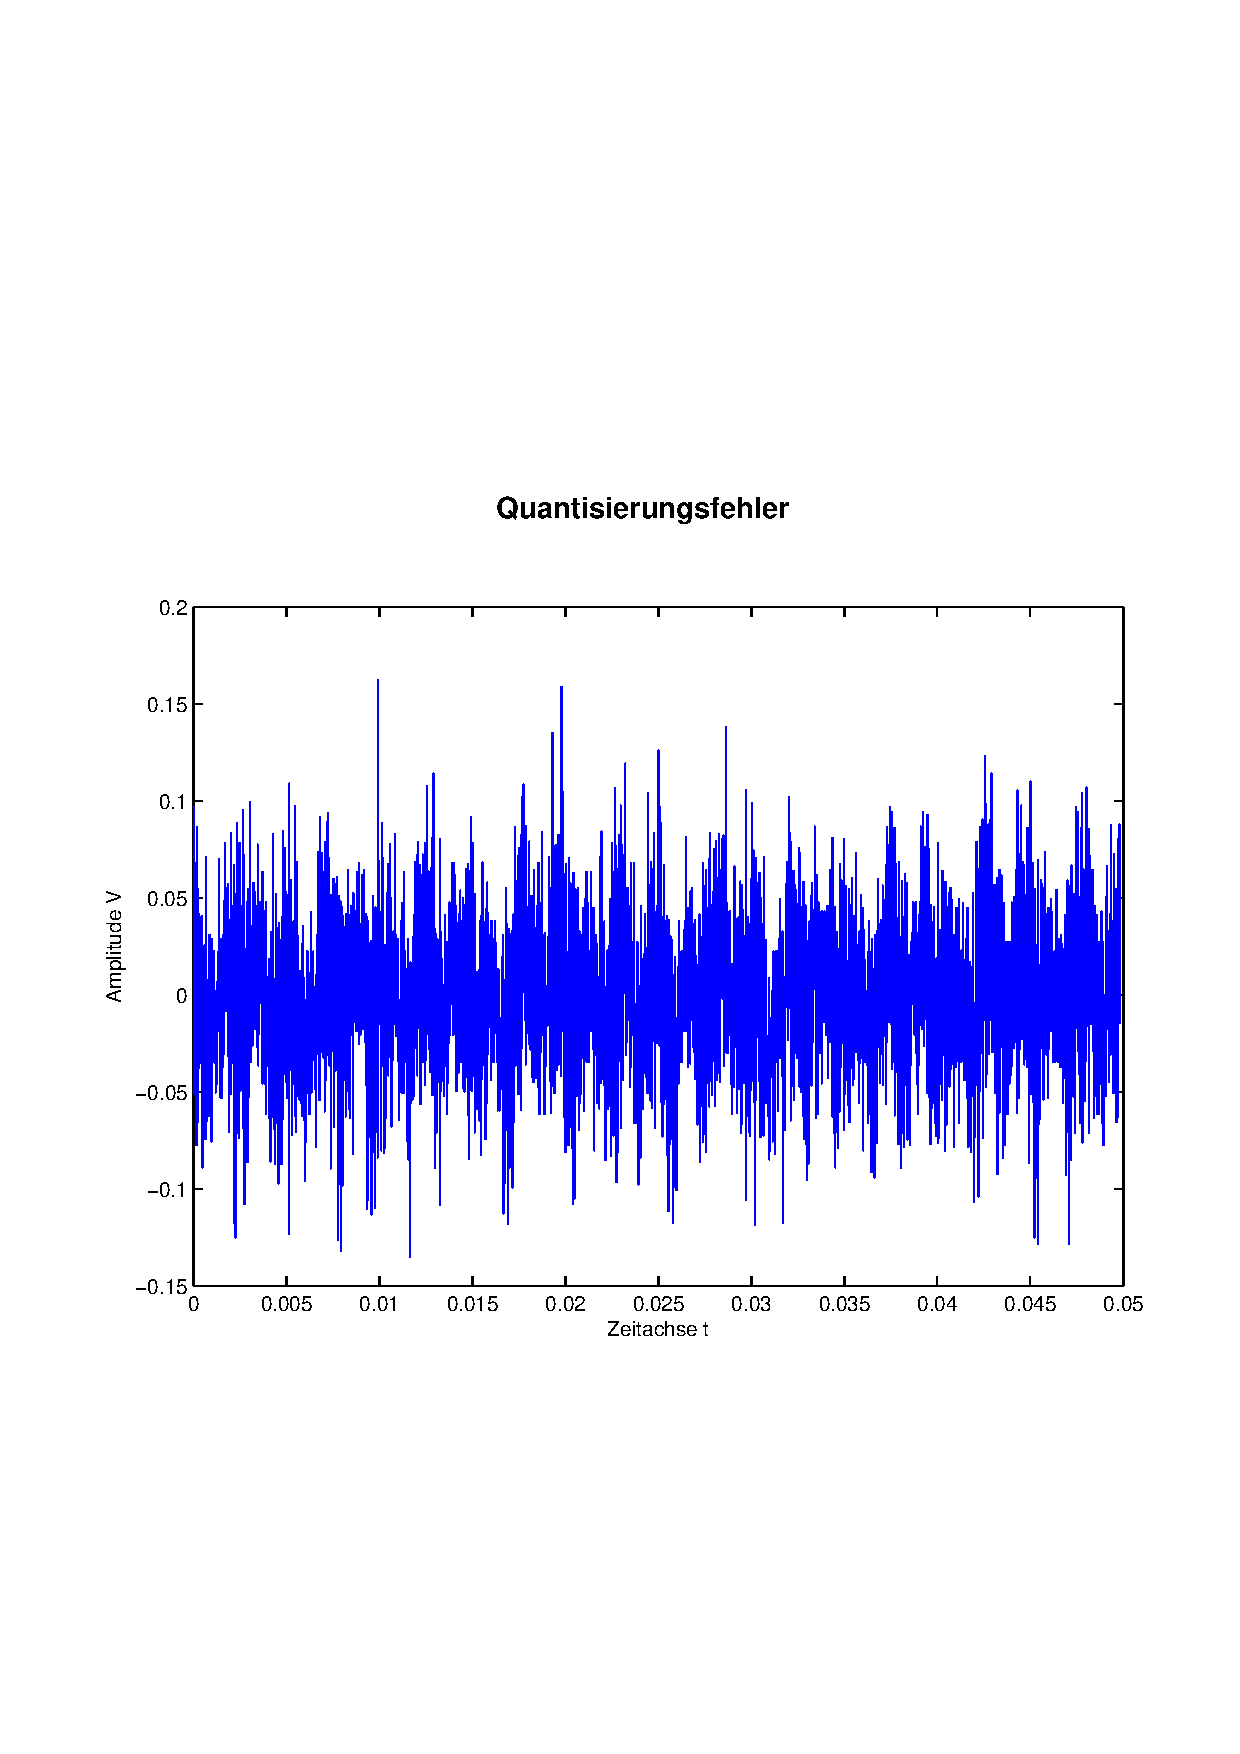
\includegraphics[scale=0.4, trim = 0cm 7cm 0cm
                            7.5cm, clip]
                            {./Bilder/sin100_Quantisierungsfehler}
                              \caption{Quntisierungsfehler (Sinus, 100kHz clk)}
                        \end{figure}
                    \end{minipage}
                                  
                    \begin{minipage}{0.6\textwidth}
                        \begin{figure}[H]
                            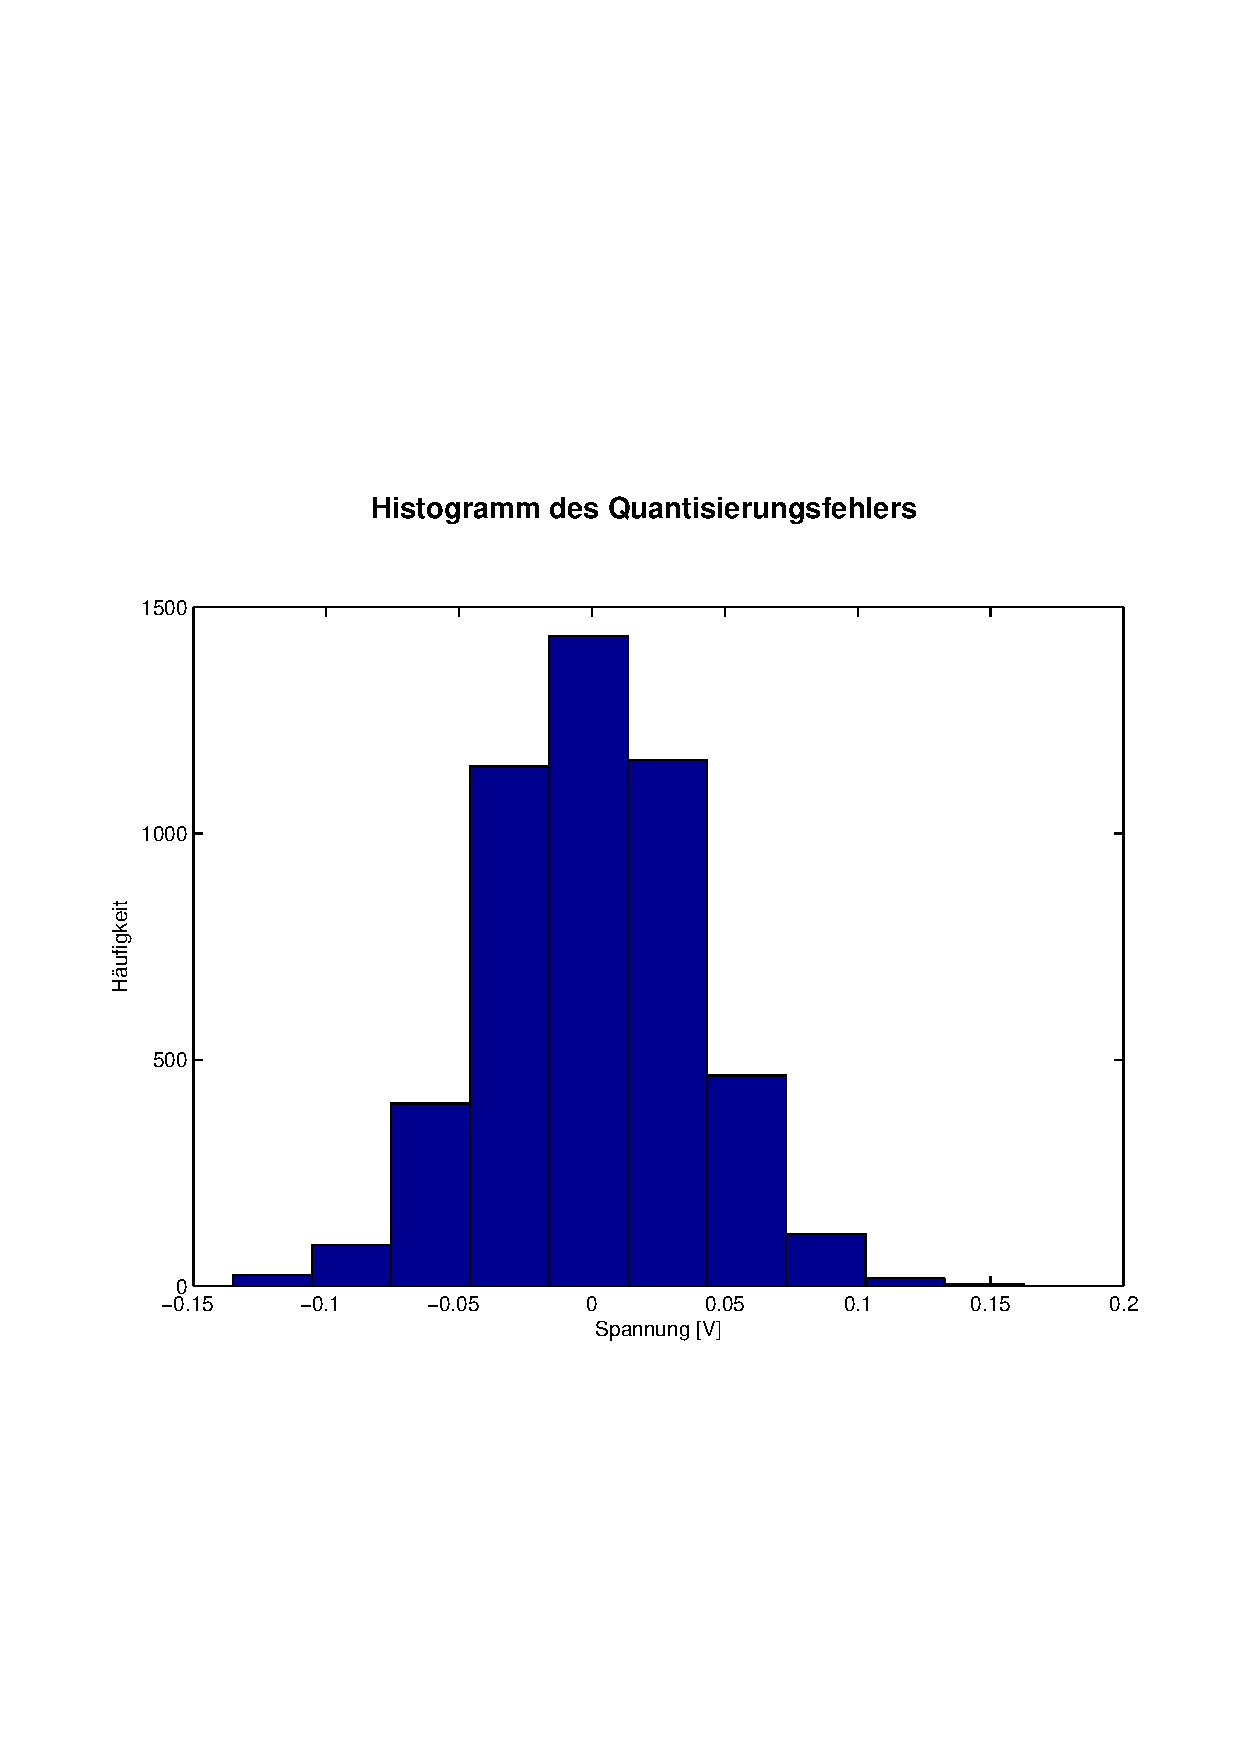
\includegraphics[scale=0.4, trim = 0cm 7cm 0cm
                            7.5cm, clip]
                            {./Bilder/sin100_Histogramm}
                              \caption{Histogramm des Quantisierungsfehlers}
                        \end{figure}
                    \end{minipage}
                
                \end{tabular}
            \end{center}
            \vspace{1em}
            
            \TODO{Plots erklären, was zum Quantisierungsfehler sagen}
            
            \vspace{1em}
            
            Nun betrachten wir das Dreiecksignal. Wie oben beginnen wir bei einer Abtastfrequenz von $8 kHz$.
            
            \begin{center}
                \begin{tabular}{ll}
                
                \hspace{-4cm}
                    \begin{minipage}{0.6\textwidth}
                        \begin{figure}[H]
                            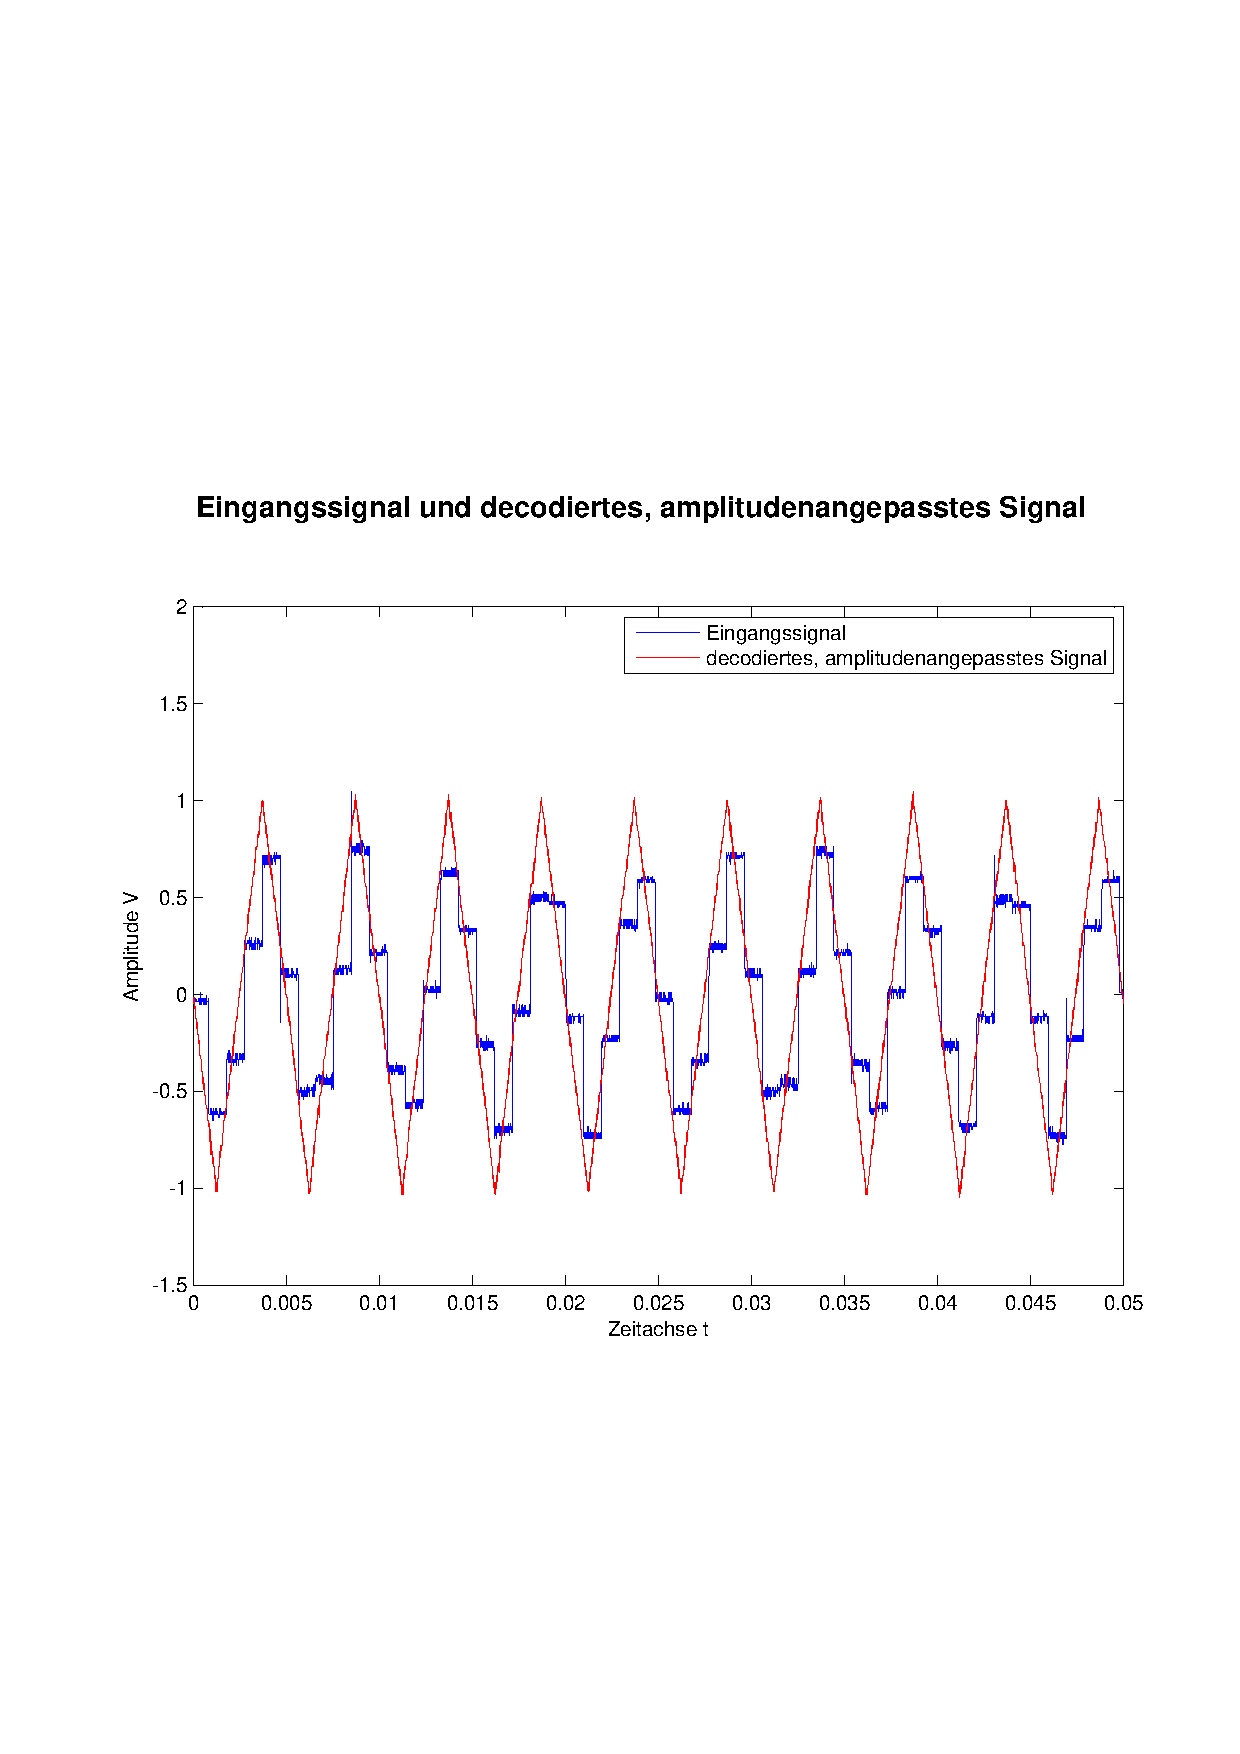
\includegraphics[scale=0.4, trim = 0cm 7cm 0cm
                            7.5cm, clip]
                            {./Bilder/drei8_Eingang_vs_DecodiertAmpl-angepasst}
                              \caption{Eingangssignal und decodiert, \newline
                              amplitudenangepasstes Signal}
                        \end{figure}
                    \end{minipage}
                    
                    \begin{minipage}{0.6\textwidth}
                        \begin{figure}[H]
                            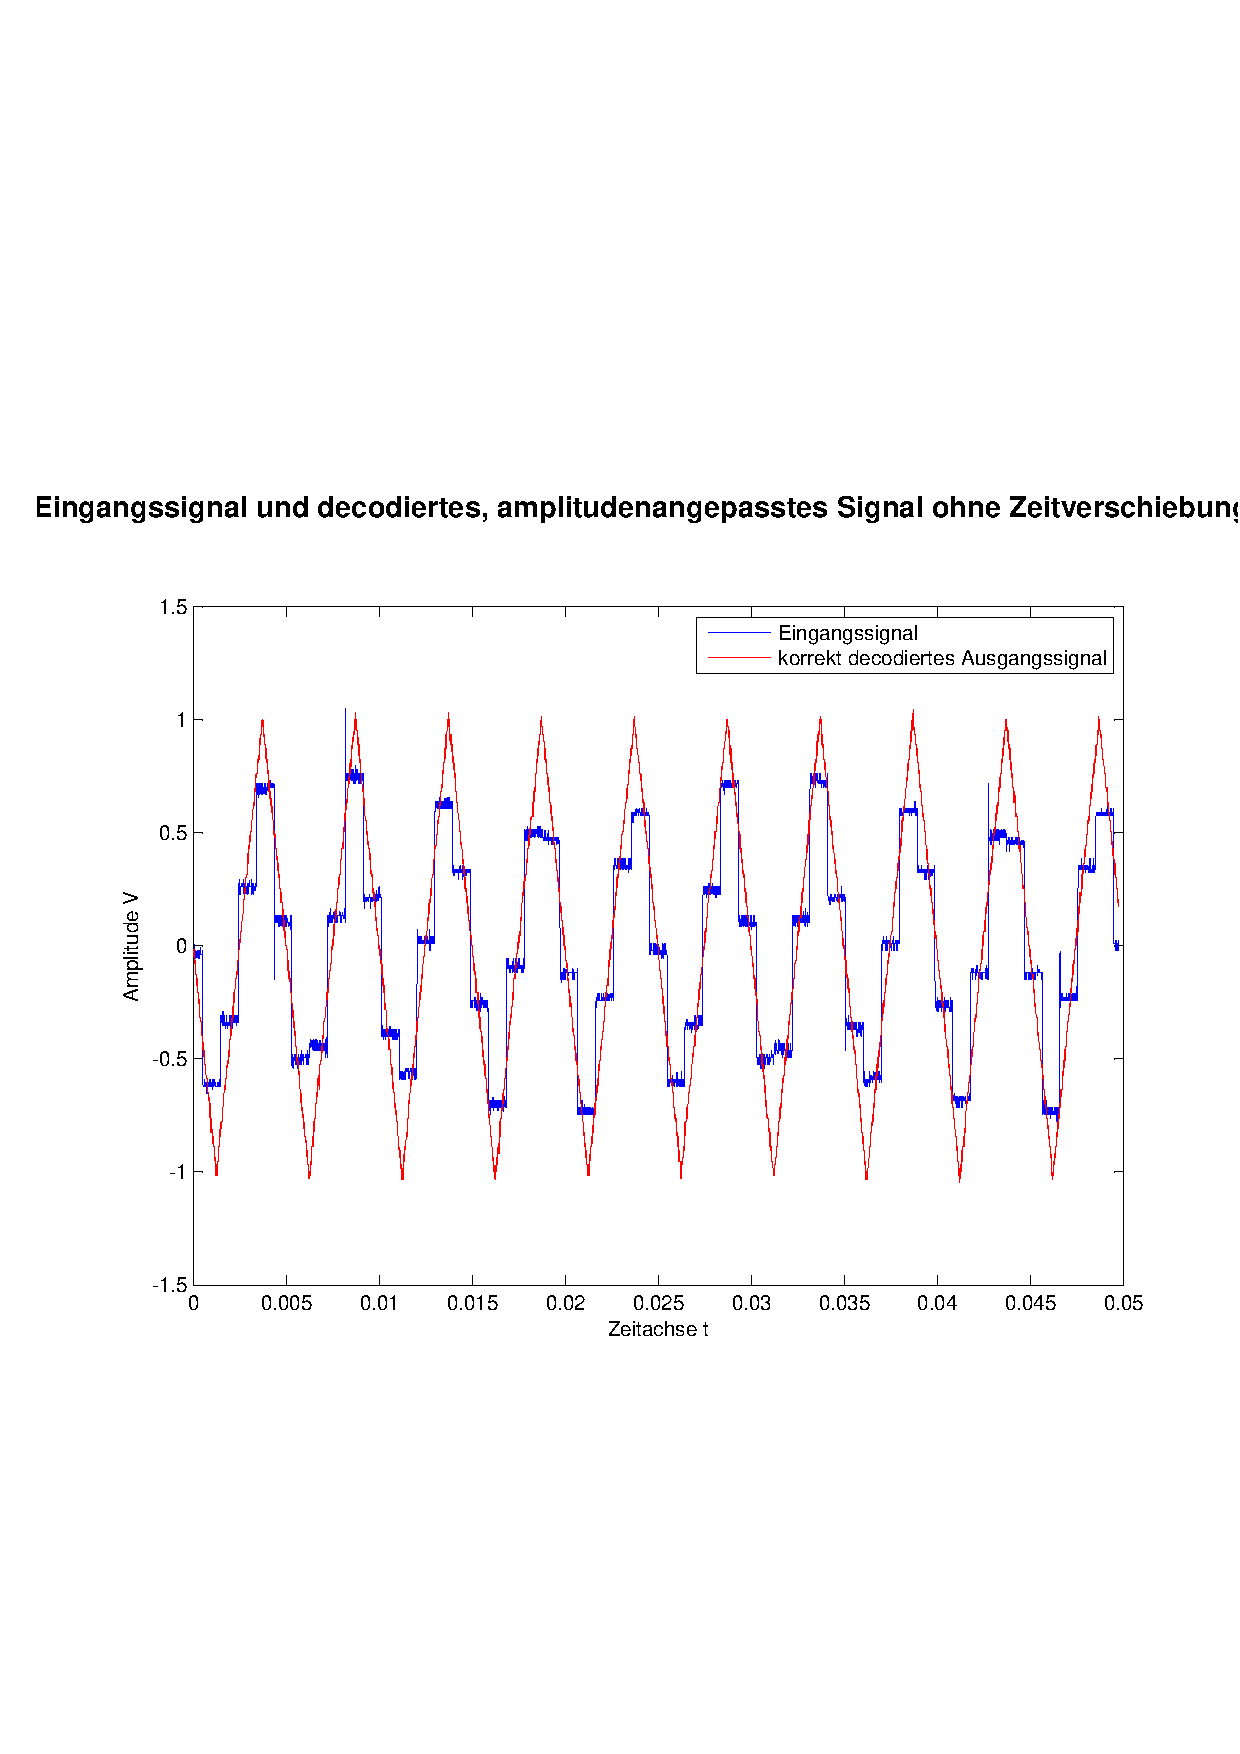
\includegraphics[scale=0.4, trim = 0cm 7cm 0cm
                            7.5cm, clip]
                            {./Bilder/drei8_Eingang_vs_korrektDecodiert}
                              \caption{Eingangssignal und korrekt decodiertes
                              Ausgangssignal}
                        \end{figure}
                    \end{minipage}
                
                \end{tabular}
            \end{center}
            
            
            
            \begin{center}
                \begin{tabular}{ll}
                
                \hspace{-4cm}
                    
                    \begin{minipage}{0.55\textwidth}
                        \begin{figure}[H]
                            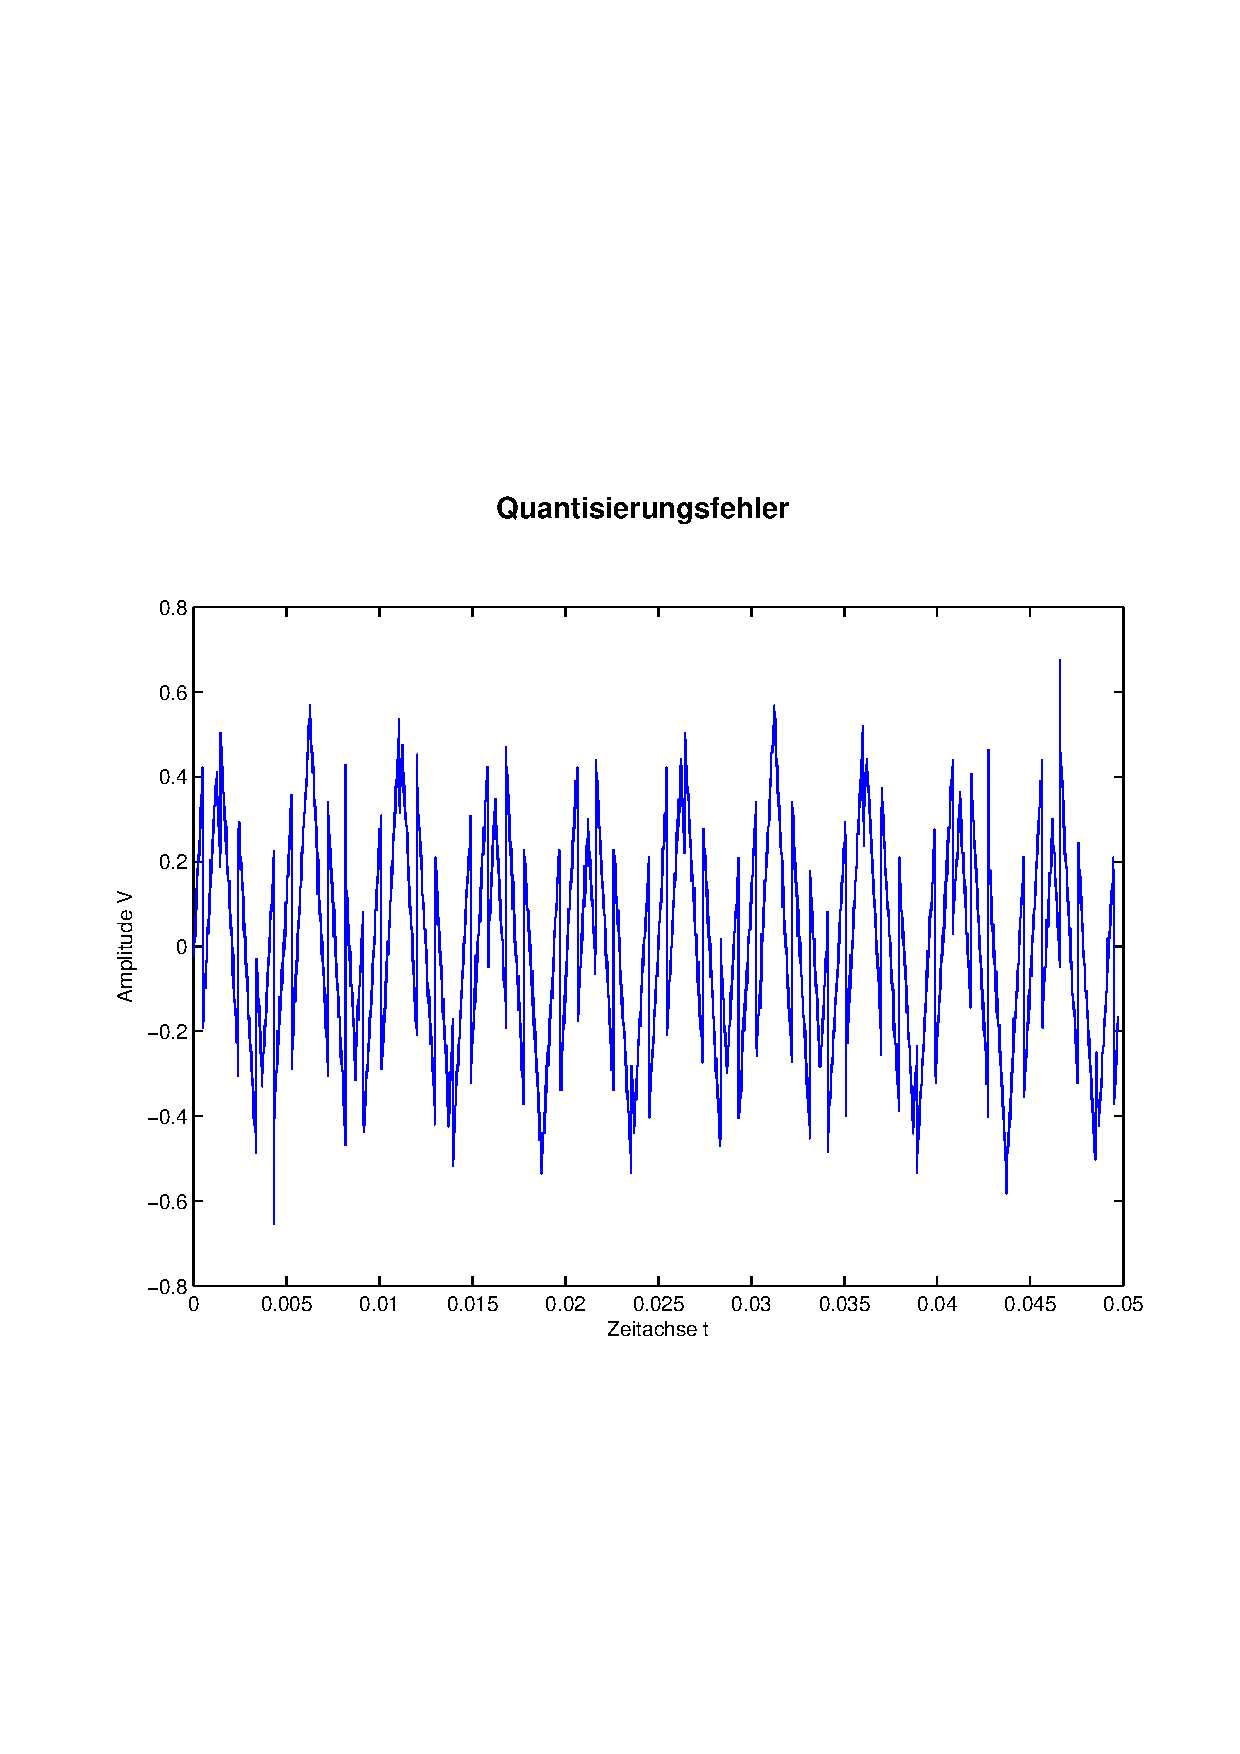
\includegraphics[scale=0.4, trim = 0cm 7cm 0cm
                            7.5cm, clip]
                            {./Bilder/drei8_Quantisierungsfehler}
                              \caption{Quntisierungsfehler (Dreieck, 100kHz clk)}
                        \end{figure}
                    \end{minipage}
                                  
                    \begin{minipage}{0.6\textwidth}
                        \begin{figure}[H]
                            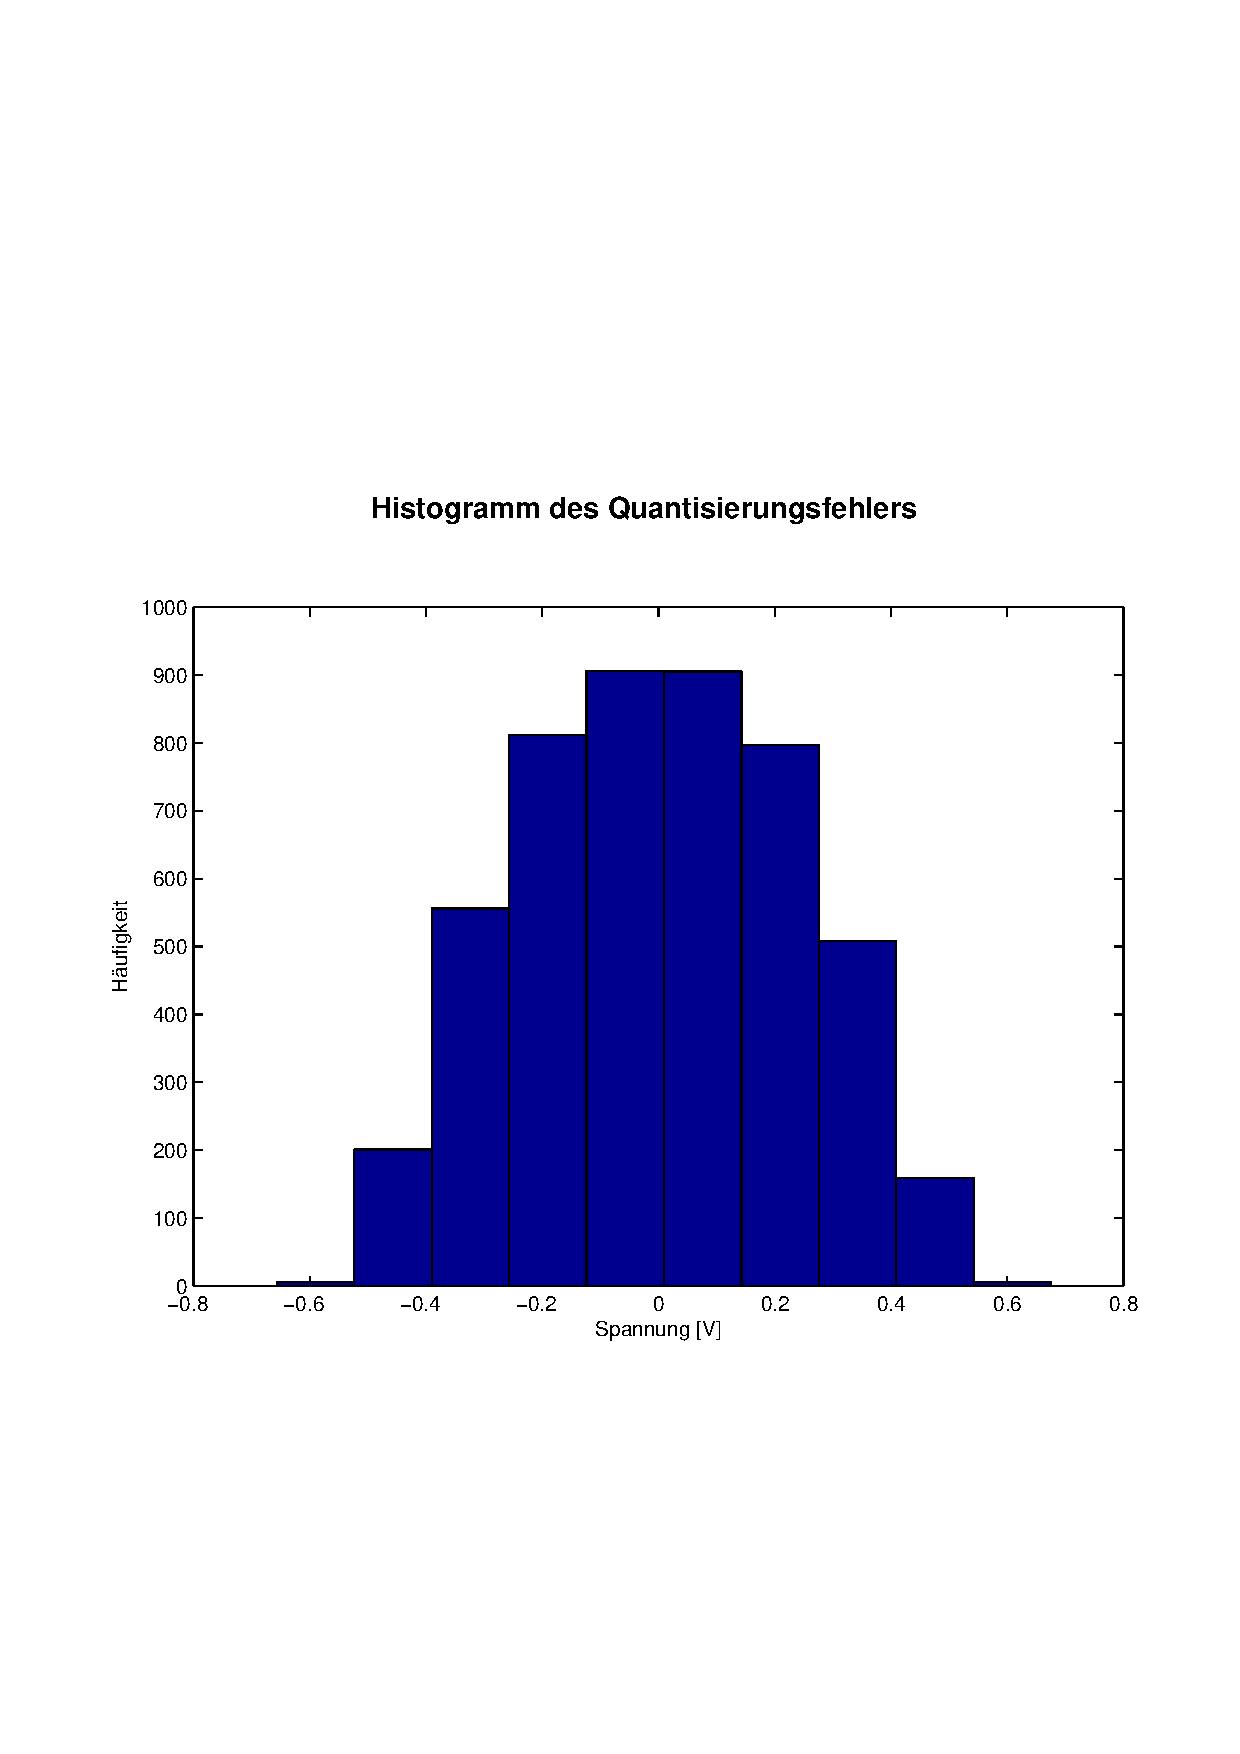
\includegraphics[scale=0.4, trim = 0cm 7cm 0cm
                            7.5cm, clip]
                            {./Bilder/drei8_Histogramm}
                              \caption{Histogramm des Quantisierungsfehlers}
                        \end{figure}
                    \end{minipage}
                
                \end{tabular}
            \end{center}
            \vspace{1em}
            
            \TODO{Plots erklären, was zum Quantisierungsfehler sagen}        
            
            
            \vspace{1em}
            
            Als letztes widmen wir uns dem Dreiecksignal bei der Abtstfrequenz $100 kHz$.

            \begin{center}
                \begin{tabular}{ll}
                
                \hspace{-4cm}
                    \begin{minipage}{0.6\textwidth}
                        \begin{figure}[H]
                            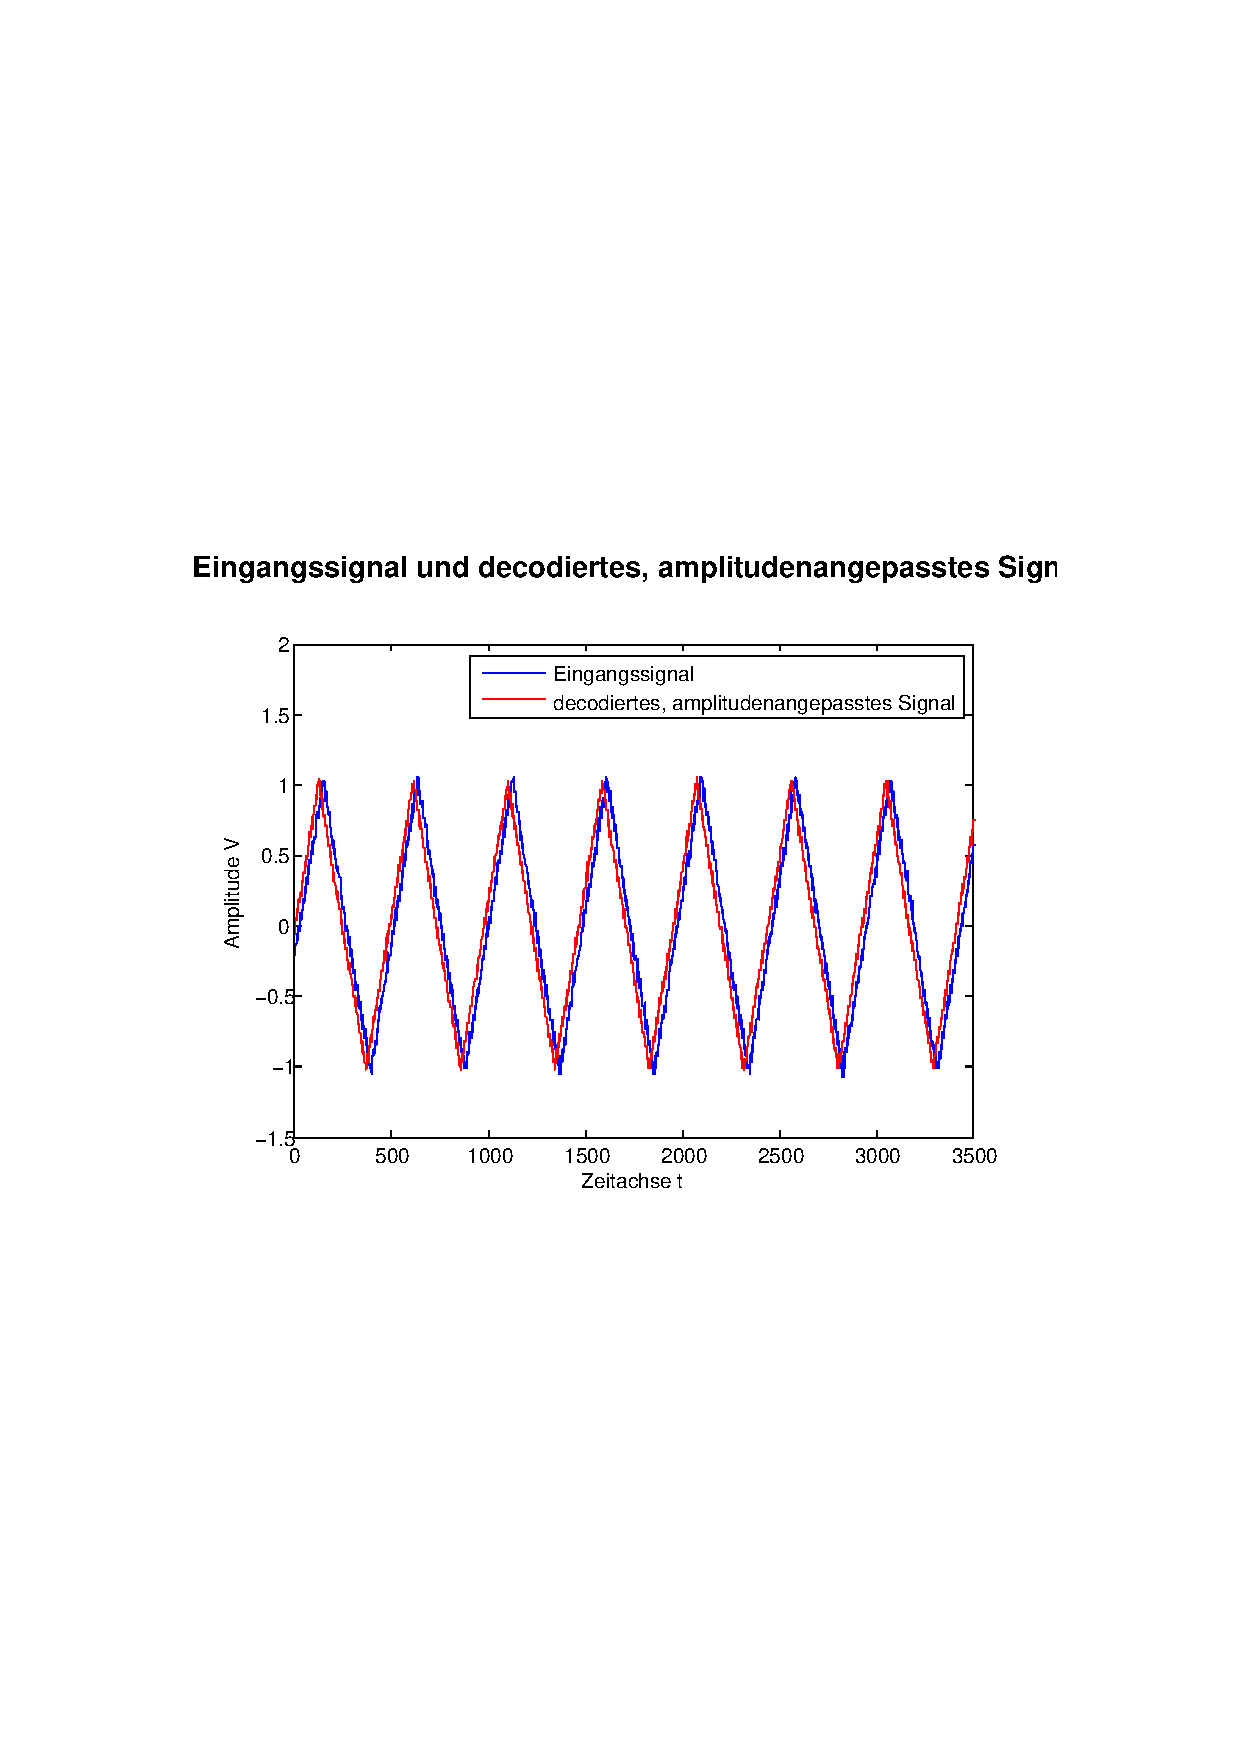
\includegraphics[scale=0.4, trim = 0cm 7cm 0cm
                            7.5cm, clip]
                            {./Bilder/drei100_Eingang_vs_DecodiertAmpl-angepasst}
                              \caption{Eingangssignal und decodiert, \newline
                              amplitudenangepasstes Signal}
                        \end{figure}
                    \end{minipage}
                    
                    \begin{minipage}{0.6\textwidth}
                        \begin{figure}[H]
                            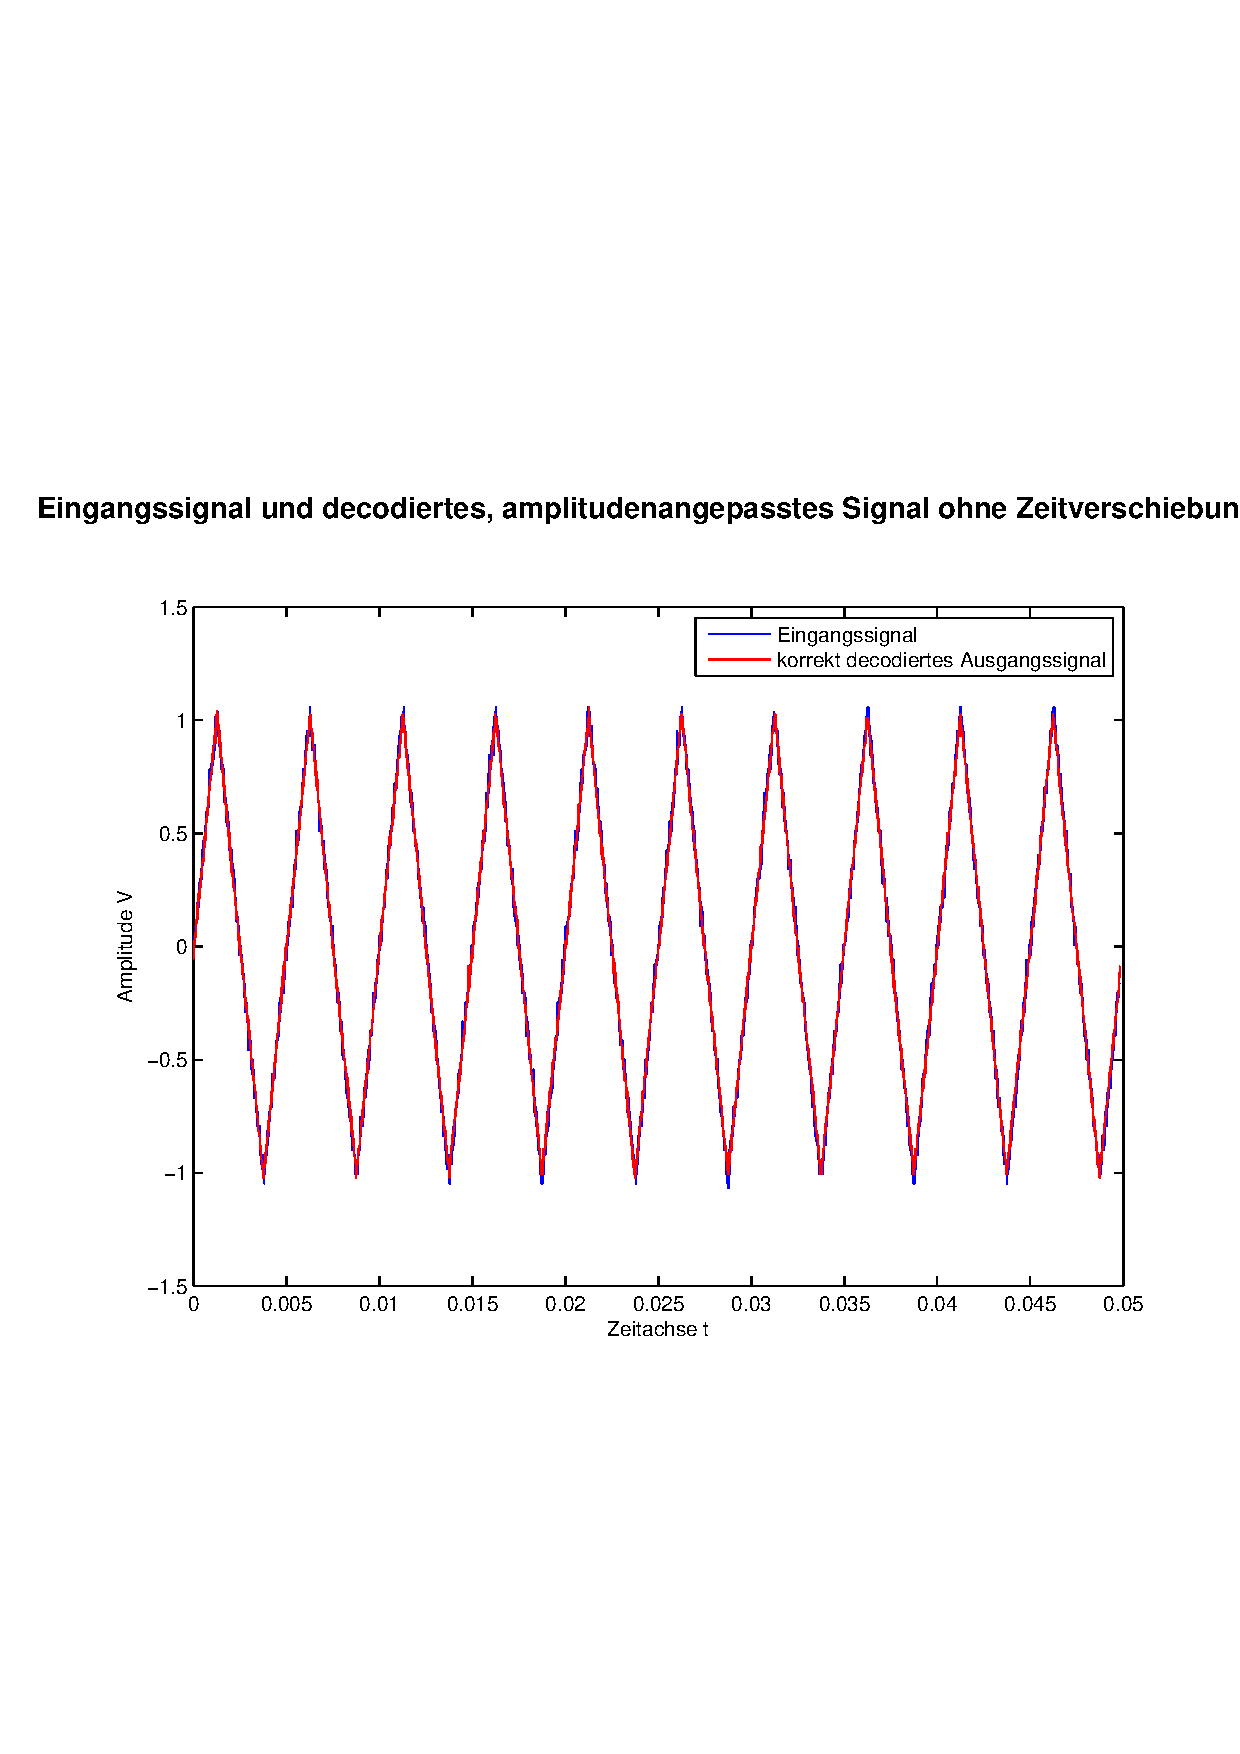
\includegraphics[scale=0.4, trim = 0cm 7cm 0cm
                            7.5cm, clip]
                            {./Bilder/drei100_Eingang_vs_korrektDecodiert}
                              \caption{Eingangssignal und korrekt decodiertes
                              Ausgangssignal}
                        \end{figure}
                    \end{minipage}
                
                \end{tabular}
            \end{center}
            
            
            
            \begin{center}
                \begin{tabular}{ll}
                
                \hspace{-4cm}
                    
                    \begin{minipage}{0.55\textwidth}
                        \begin{figure}[H]
                            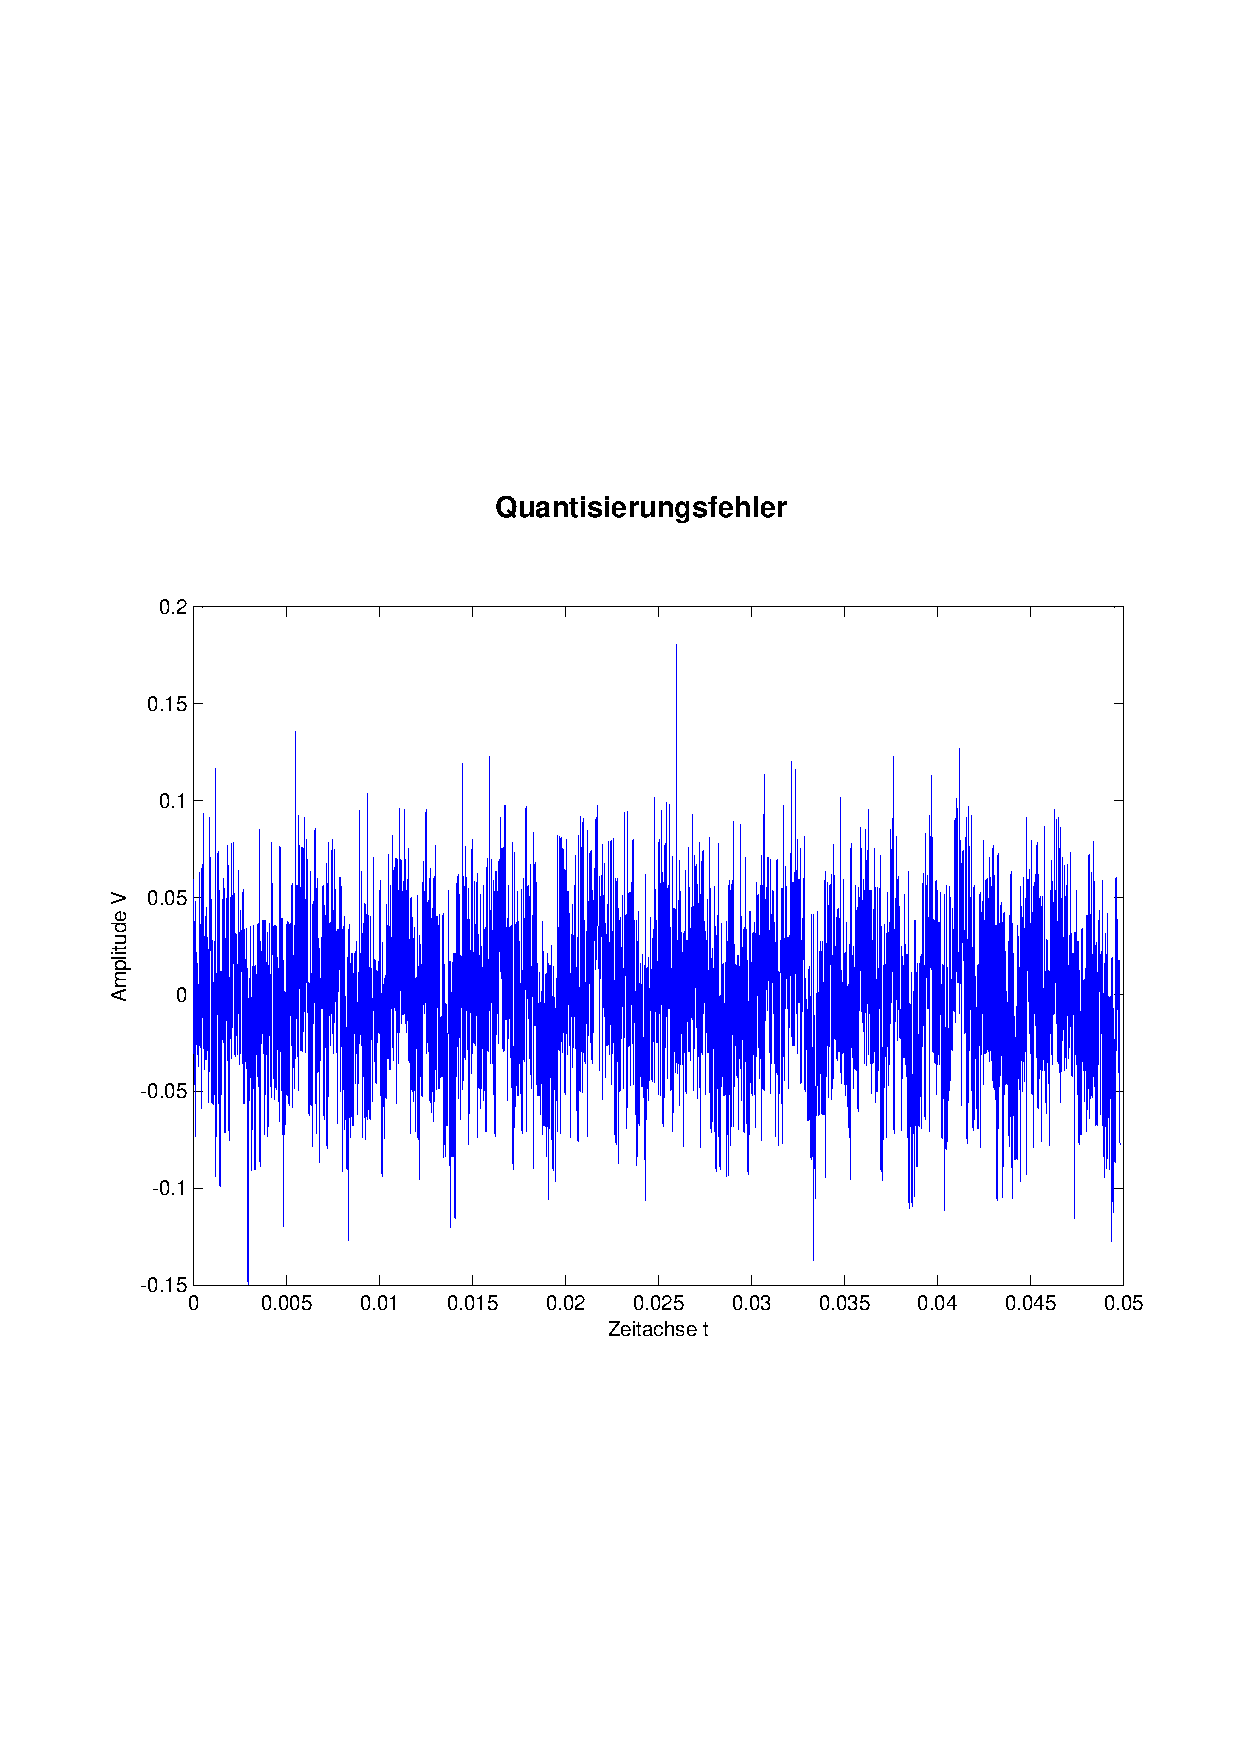
\includegraphics[scale=0.4, trim = 0cm 7cm 0cm
                            7.5cm, clip]
                            {./Bilder/drei100_Quantisierungsfehler}
                              \caption{Quntisierungsfehler (Dreieck, 100kHz clk)}
                        \end{figure}
                    \end{minipage}
                                  
                    \begin{minipage}{0.6\textwidth}
                        \begin{figure}[H]
                            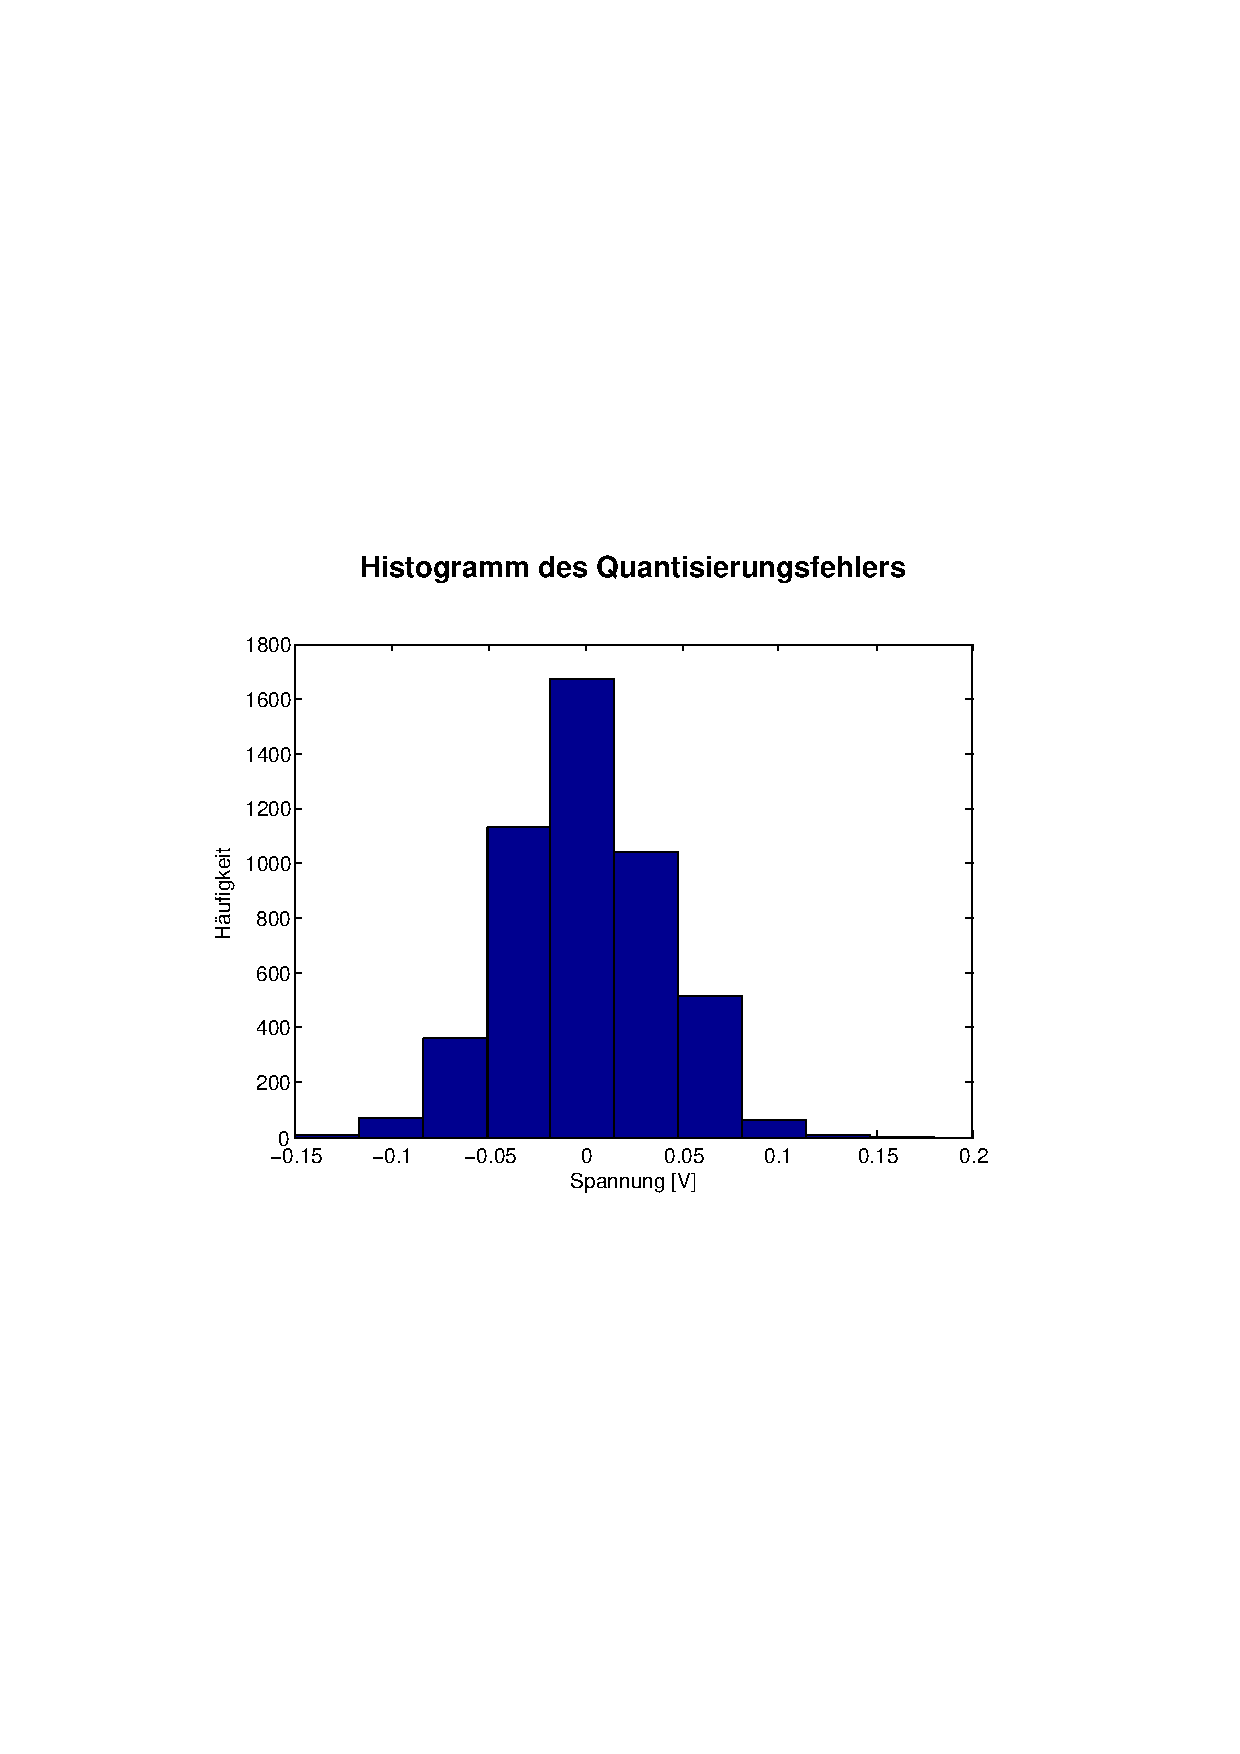
\includegraphics[scale=0.4, trim = 0cm 7cm 0cm
                            7.5cm, clip]
                            {./Bilder/drei100_Histogramm}
                              \caption{Histogramm des Quantisierungsfehlers}
                        \end{figure}
                    \end{minipage}
                
                \end{tabular}
            \end{center}
            \vspace{1em}
            
            \TODO{Plots erklären, was zum Quantisierungsfehler sagen}
        
        \end{quote}  % Ende Subsection Quantisierungsfehler und Histogram
        
        \subsubsection{Leistungsdichtespektrum des Quantisierungsfehlers}
		\begin{quote}
		
		Ein Leistungsdichtespektrum beschreibt die Verteilung der Leistung über der Frequenz und wird als
		Fouriertransformation der Autokorrelationsfunktion eines stationären stochastischen Prozesses definiert.\cite{LDS}\\
		Für diesen Versuch errechenen wir das LDS das eben berechneten Quantisierungsrauschen. 

        \begin{center}
            \begin{tabular}{ll}
            
            \hspace{-4cm}
                
                \begin{minipage}{0.55\textwidth}
                    \begin{figure}[H]
                        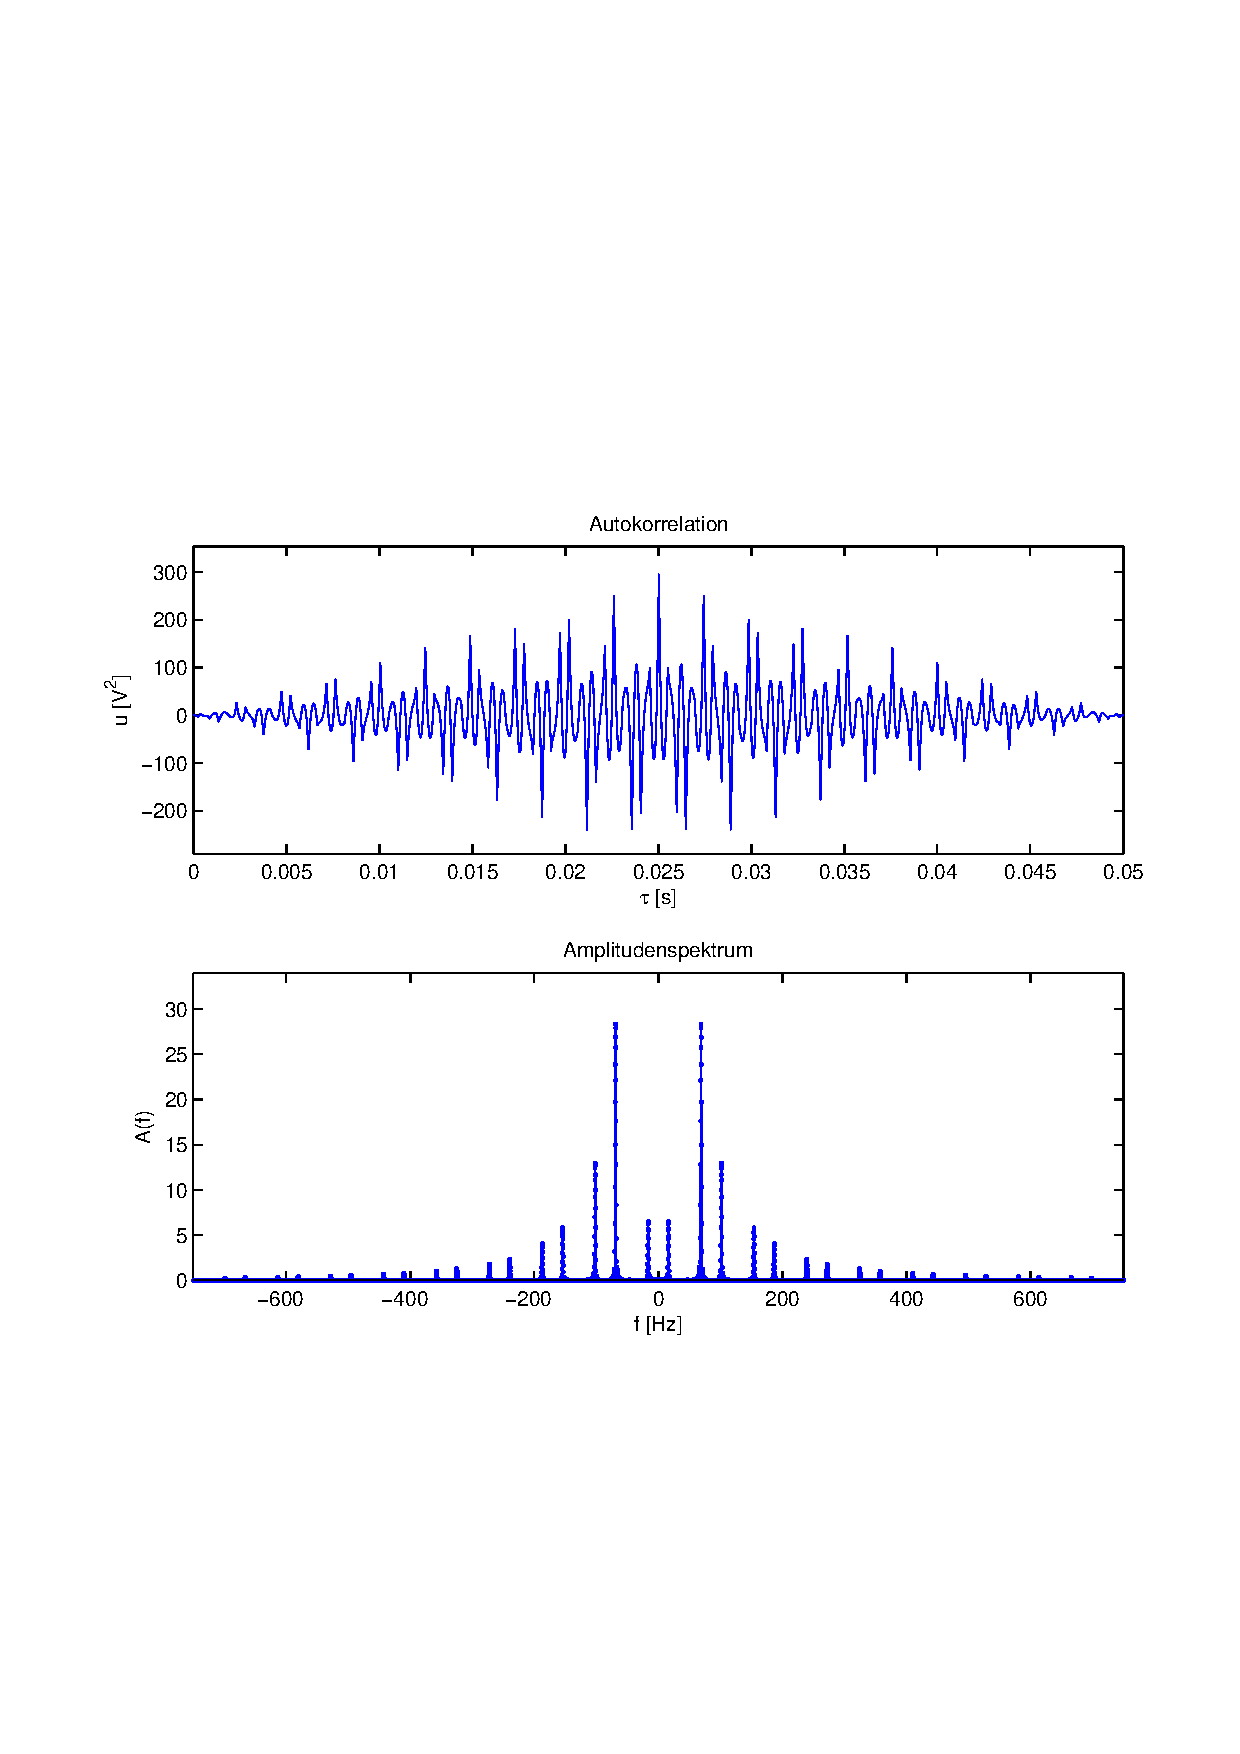
\includegraphics[scale=0.4, trim = 1.5cm 7cm 1.5cm 8cm, clip]
                        {./Bilder/sin8_Quantisierungsfehler_LDS}
                          \caption{LDS - Sinussignal 8kHz}
                    \end{figure}
                \end{minipage}
                              
                \begin{minipage}{0.6\textwidth}
                    \begin{figure}[H]
                        
\includegraphics[scale=0.4, trim = 1.5cm 7cm 1.5cm 8cm, clip]
                        {./Bilder/sin100_Quantisierungsfehler_LDS}
                          \caption{LDS - Sinussignal 100kHz}
                    \end{figure}
                \end{minipage}
            
            \end{tabular}
        \end{center}
        
                \begin{center}
            \begin{tabular}{ll}
            
            \hspace{-4cm}
                
                \begin{minipage}{0.55\textwidth}
                    \begin{figure}[H]
                        \includegraphics[scale=0.4, trim = 1.5cm 7cm 1.5cm 8cm, clip]
                        {./Bilder/drei8_Quantisierungsfehler_LDS}
                          \caption{LDS - Dreiecksignal 8kHz}
                    \end{figure}
                \end{minipage}
                              
                \begin{minipage}{0.6\textwidth}
                    \begin{figure}[H]
                        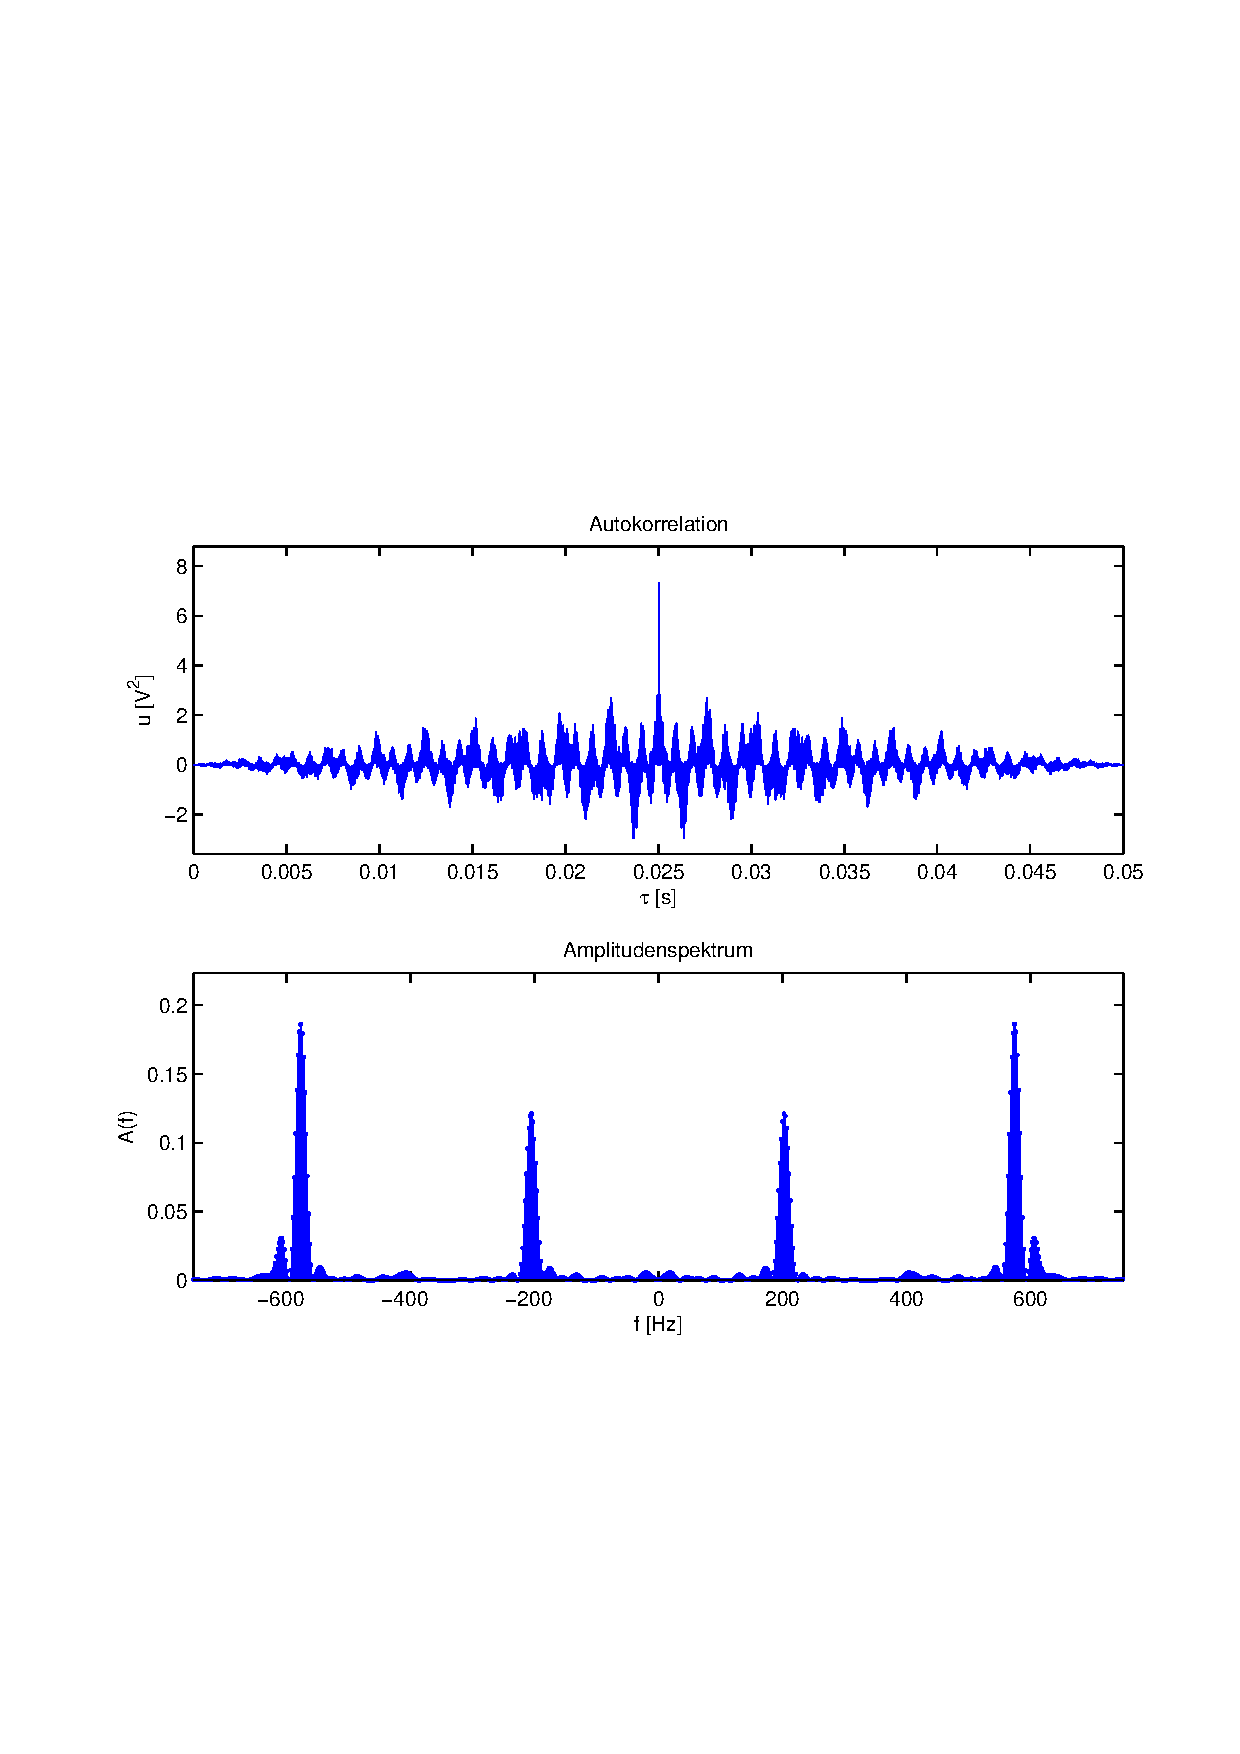
\includegraphics[scale=0.4, trim = 1.5cm 7cm 1.5cm 8cm, clip]
                        {./Bilder/drei100_Quantisierungsfehler_LDS}
                          \caption{LDS - Dreiecksignal 100kHz}
                    \end{figure}
                \end{minipage}
            
            \end{tabular}
        \end{center}
        \vspace{1em}
			
		Bei beiden Signalentypen, Sinus und Dreiecksignal, fällt auf, dass das Leistungsdichtespektrum des
		Quantisierungsfehlers bei den Messungen mit einer Abtastrate von $8 kHz$ deutlich höher ist als bei der Abtastrate
		$100 kHz$. Das lässt auf einen wesentlich höheres Quantisierungrauschen bei der niedrigereren Abtastrate schließen und
		passt daher zu unserern Beobachtungen auf der vorhergehenden Aufgabe.
			
		\end{quote} % Ende Subsubsection LDS
    \end{quote}  % Ende Subsection Quantisierungsfehler
         	
\end{quote}%beende Auswertung

%--------------------------------------------------------------------
%-------------------------------------------------------------------- 
    
\section{Zusammenfassung}
\begin{quote}

    \TODO{Zusammenfassug schreiben} \\
\end{quote}%beende Zusammenfassung
         

%--------------------------------------------------------------------
%--------------------------------------------------------------------    


\begin{thebibliography}{999}
 \bibitem {PCM-Uebertragung} Prof. Dr.-Ing. Sikora, Thomas; Prof. Dr.-Ing. Noll, Peter: Einführung in die
 Nachrichtenübertragung, S.272
\bibitem {Digitalisierung_des_Signals} Prof. Dr.-Ing. Sikora, Thomas; Prof. Dr.-Ing. Noll, Peter: Einführung in die
 Nachrichtenübertragung, S.273
\bibitem {PCM_Decodierung} Prof. Dr.-Ing. Sikora, Thomas; Prof. Dr.-Ing. Noll, Peter: Einführung in die
 Nachrichtenübertragung, S.276
 \bibitem {LDS} Prof. Dr.-Ing. Sikora, Thomas; Prof. Dr.-Ing. Noll, Peter: Einführung in die
 Nachrichtenübertragung, S.123-124



%Name, Vorname.; evtl. Name2, Vorname2.: Titel des Dokumentes
%oder Buches, Zeitschrift/Verlag/URL (Auflage, Erscheinungsort, -jahr), ggf. Seitenzahlen
% \bibitem {PasevalscheTheorem} \url{https://de.wikipedia.org/wiki/Parsevalsches_Theorem}, Zugriff
% 23.05.2012
\end{thebibliography}

\end{document}
  	    
